\documentclass[12pt,a4paper]{article}

\newcommand{\boldmark}[1]{\noindent\textbf{#1}\\ }
\usepackage{graphicx}
\usepackage[utf8]{inputenc}
\usepackage[english]{babel}
\newcommand{\sol}[1]{#1}
\setlength{\textheight}{25.5cm}
\usepackage{setspace}
\usepackage{amssymb}
\usepackage{amsmath}
\usepackage{fancyhdr}
\usepackage{lastpage}
\usepackage{multirow}
\usepackage{xcolor}
\usepackage{placeins}
\usepackage{float}
\usepackage{rotating}
\usepackage{algorithm2e}
\SetKwComment{Comment}{/* }{ */}
\RestyleAlgo{ruled}
\pagestyle{fancy}
\fancyhf{}
\renewcommand{\baselinestretch}{1.1}
\renewcommand{\headrulewidth}{0pt}
\usepackage[legalpaper, margin=1in]{geometry}
\DeclareSymbolFont{matha}{OML}{txmi}{m}{it}
\DeclareMathSymbol{\varv}{\mathord}{matha}{118}
\cfoot{\hspace{70pt} Page \thepage \hspace{1pt} of \pageref{LastPage}}
\usepackage{enumitem}
\setlist[itemize] {leftmargin=1.8em}
\definecolor{crimsonglory}{rgb}{0.75, 0.0, 0.2}
\usepackage{hyperref}

\begin{document}


\begin{titlepage}

	\begin{center}

		
\includegraphics[scale=0.5] {tuc_logo_text.png} \\[3cm]

		\large
		\rule{0.8\textwidth}{2pt} \\[0.5cm]
		
		\textbf{\Large{Gaussian Process Regression}} \\[0.5cm]
		\textbf{\Large{An application on sunspots data-set}} \\[1.5cm]
		{\Large{Exercise Report}} \\[0.1cm]
		\rule{0.8\textwidth}{2pt} \\[4cm]
		
		\begin{tabular}{l l}
		    \large{Professor:} & \large{Dionysios Christopoulos}\\\\
			\large{Student:} & \large{Nikolaos Paraskakis} \\
			\large{I.D.:} & \large{2018030027} \\
		\end{tabular}
		
		\vspace{5cm}
		\textmd{\large{SCHOOL OF ELECTRICAL \& COMPUTER ENGINEERING}} \\[0.5cm]
		\today \\
		
	\end{center}
		
\end{titlepage}



%%%%%%%%%%%%%%%%%%%%%%%%%%%%%%%%%          1          %%%%%%%%%%%%%%%%%%%%%%%%%%%%%%%%%%%%%%

\sectionmark{}
\noindent
\boldmark{\Large{{\color{crimsonglory}EXECUTIVE SUMMARY}}}

\normalsize

\begin{spacing}{1.5}
\noindent
\\In this report, we discuss the basic theory behind Gaussian Progress Regression (GPR) and how we can use that tool to build a model for curve fitting and making accurate predictions. Such a model, has the advantage that is probabilistic and can give us also information of uncertainty in our predictions, unlike other deterministic regression models.

\noindent
\\In this context, we describe the importance of kernel (covariance) function's selection, along with the tuning of its hyperparameters, in order to achieve the optimal behavior of our model. A popular approach to this is by using Bayesian optimization in a purpose of maximizing the log marginal likelihood. We use cross-validation for training and testing our GPR model. As for this partitioning over our original data-set, we explore the benefits of applying it in a more intelligent way rather than a random. Also, we examine the impact of normalization of the original data-set in the final performance. Finally, RRMSE is chosen as a metric to evaluate the performance-accuracy of the trained GPR model.

\noindent
\\As far as the implementation and experiment are concerned, a data-set containing the yearly mean total sunspot number from $1700$ until now is being used in order to practice GPR on it. After presenting some result evidence, we conclude that a very good performance can be achieved by using ``Ard Matern 3/2" kernel function. It gives very small RRMSE and strict prediction intervals of $95\%$ confidence level. We do not use normalization of the original data-set and for the training we use the $90\%$ of it, while holding out the rest $10\%$ for cross-validation (testing). As said before, this partition is being done not randomly, but in a way that the training set includes the turning points (peaks) of the observed data in an attempt of developing a better model.

\end{spacing}

\newpage

\sectionmark{}
\noindent
\boldmark{\Large{{\color{crimsonglory}INTRODUCTION}}}

\normalsize

\noindent
In this exercise, the purpose is to experiment with Gaussian Process Regression (GPR) models and use them as tools for curve fitting. At our disposal, we have a data-set containing the yearly mean total sunspot number from $1700$ until now and we will practice GPR on it. In particular, we build a model that fits the observed data as much as possible and at the same time is capable of making accurate predictions on unobserved (new) data-points. As we will discuss below, there are several decisions that need to be made and hyperparameters that need to be tuned in such a model. In this context, we explore some of the most significant parameters of a GPR model and we evaluate its performance while testing various such choices.

\vspace{1.5cm}

\sectionmark{}
\noindent
\boldmark{\Large{{\color{crimsonglory}DISCUSSION}}}

\vspace{0.5cm}

\subsectionmark{}
\noindent
\boldmark{\large{Theoretical background}}

\normalsize

\noindent
Gaussian Process Regression (GPR) models are \textbf{non-parametric} kernel-based \textbf{probabilistic} models. Gaussian Process (GP) is considered non-parametric because a GP represents a function, i.e. an infinite dimensional vector. More specific, as the number of data-points increases ($(\mathbf{x}, f(\mathbf{x}))$ pairs), so do the number of model parameters restricting the shape of the function.

\noindent
\\Consider the training set $D = \{(\mathbf{x}_i,y_i), i = 1,2,\dots,n\}$, where $\mathbf{x}_i \in \mathbb{R}^{d}$ and $y_i \in \mathbb{R}$. A GPR model addresses the question of predicting the value of a response variable $y_{*}$, given the new input vector $\mathbf{x}_{*}$, and the training data. Generally, in regression, there is a function $f$ we are trying to model given the observed data points $D$.

\noindent
\\We assume that the entire function evaluation, associated with the observed data points D, is a draw from a Multi-Variate Gaussian (MVG) distribution. This is the \textbf{prior distribution} and it holds that
$$
p(\mathbf{y}(\mathbf{x}))=\mathcal{N}(\boldsymbol{\mu}(\mathbf{x}),\mathbf{K}(\mathbf{x},\mathbf{x}))
$$
where $\mathbf{y} = \begin{bmatrix} y_1 & y_2 & \dots & y_n\\ \end{bmatrix}^{T}$ are the dependent function values, evaluated at locations $\mathbf{x} = \begin{bmatrix} \mathbf{x}_1 & \mathbf{x}_2 & \dots & \mathbf{x}_n\\ \end{bmatrix}^{T}$, $\boldsymbol\mu(\mathbf{x}) = \begin{bmatrix} \mu(\mathbf{x}_1) & \mu(\mathbf{x}_2) & \dots & \mu(\mathbf{x}_n)\\ \end{bmatrix}^{T}$ is a mean function, and $\mathbf{K}$ is the covariance matrix defined as:
$$
\mathbf{K}(\mathbf{x},\mathbf{x}) =
\begin{bmatrix}
k(\mathbf{x}_1,\mathbf{x}_1) & k(\mathbf{x}_1,\mathbf{x}_2) & \ldots & k(\mathbf{x}_1,\mathbf{x}_n)\\
k(\mathbf{x}_2,\mathbf{x}_1) & k(\mathbf{x}_2,\mathbf{x}_2) & \ldots & k(\mathbf{x}_2,\mathbf{x}_n)\\
\vdots & \vdots & \vdots & \vdots\\
k(\mathbf{x}_n,\mathbf{x}_1) & k(\mathbf{x}_n,\mathbf{x}_2) & \ldots & k(\mathbf{x}_n,\mathbf{x}_n)\\
\end{bmatrix}
$$
with $k(\mathbf{x}_i,\mathbf{x}_j)$ be the covariance kernel function, which provides the covariance element between any two (arbitrary) sample locations, $\mathbf{x}_i$ and $\mathbf{x}_j$. Matrix $\mathbf{K}$ has to be positive semi-definite and symmetric. 

\noindent
\\We will use the notation
$$
f \sim \mathcal{GP}(\boldsymbol\mu,\mathbf{K})
$$
to express that the function $f(\mathbf{x})$ is distributed according to a Gaussian Process (GP) with mean $\boldsymbol\mu(\mathbf{x})$ and covariance $\mathbf{K}(\mathbf{x},\mathbf{x})$.

\noindent
\\GPs encode prior distributions over functions or models and can be updated to form posterior distributions given new observed data.

\newpage

\noindent
If we believe that there is noise associated with the observed function values, $\mathbf{y}$,then we may fold this noise term into the covariance. As we expect noise to be uncorrelated from
sample to sample in our data, so the noise term adds only to the diagonal of matrix $\mathbf{K}$, giving a modified covariance for noisy observations of the form
$$
\mathbf{V}(\mathbf{x},\mathbf{x}) = \mathbf{K}(\mathbf{x},\mathbf{x}) + \sigma^2\mathbf{I}
$$
where $\mathbf{I}$ is the identity matrix of size $n \times n$ and $\sigma^2$ is a hyperparameter representing the noise variance.

\noindent
\\Let a test datum $\mathbf{x}_{*}$ and its corresponding response value $y_{*}$. The \textbf{joint distribution} of the observed data $D$, augmented by $\mathbf{x}_{*}$ and $y_{*}$ is given by:
$$
p\left(\begin{bmatrix} \mathbf{y}\\ y_{*}\\ \end{bmatrix}\right) = \mathcal{N}\left(\begin{bmatrix} \boldsymbol\mu({\mathbf{x}})\\ \mu(\mathbf{x}_{*})\\ \end{bmatrix} ,
\begin{bmatrix}
\mathbf{K}(\mathbf{x},\mathbf{x}) & \mathbf{K}(\mathbf{x},\mathbf{x}_{*}) \\
\mathbf{K}(\mathbf{x}_{*},\mathbf{x}) & k(\mathbf{x}_{*},\mathbf{x}_{*}) \\
\end{bmatrix} \right)
$$
where $\mathbf{K}(\mathbf{x},\mathbf{x}_{*}) = \begin{bmatrix} k(\mathbf{x}_1,\mathbf{x}_{*}) & k(\mathbf{x}_2,\mathbf{x}_{*}) & \dots & k(\mathbf{x}_n,\mathbf{x}_{*})\\ \end{bmatrix}^{T}$ and $\mathbf{K}(\mathbf{x}_{*},\mathbf{x}) = \mathbf{K}(\mathbf{x},\mathbf{x}_{*})^{T}$.

\noindent
\\The \textbf{posterior distribution} over $y_{*}$ is Gaussian with mean and variance given by
$$
m_{*} = \mu(\mathbf{x}_{*}) + \mathbf{K}(\mathbf{x}_{*},\mathbf{x})\mathbf{K}(\mathbf{x},\mathbf{x})^{-1}(\mathbf{y}(\mathbf{x}) - \boldsymbol\mu(\mathbf{x}))
$$
$$
\sigma^{2}_{*} = k(\mathbf{x}_{*},\mathbf{x}_{*}) - \mathbf{K}(\mathbf{x}_{*},\mathbf{x})\mathbf{K}(\mathbf{x},\mathbf{x})^{-1}\mathbf{K}(\mathbf{x},\mathbf{x}_{*})
$$

\noindent
\\Consider the testing set $S = \{(\mathbf{x}_{*,i},y_{*,i}), i = 1,2,\dots,q\}$, where $\mathbf{x}_{*,i} \in \mathbb{R}^{d}$ and $y_{*,i} \in \mathbb{R}$. Now, we extend what we have already said to infer the GP at a set of locations outside our observations, at set $\mathbf{x}_{*}$, to evaluate the \textbf{posterior distribution} of $\mathbf{y}(\mathbf{x}_{*})$, which is given by
$$
p(\mathbf{y}_{*})=\mathcal{N}(\mathbf{m}_{*},\mathbf{\Sigma}_{*})
$$
where
$$
\mathbf{m}_{*} = \boldsymbol\mu(\mathbf{x}_{*}) + \mathbf{K}(\mathbf{x}_{*},\mathbf{x})\mathbf{K}(\mathbf{x},\mathbf{x})^{-1}(\mathbf{y}(\mathbf{x}) - \boldsymbol\mu(\mathbf{x}))
$$
$$
\mathbf{\Sigma}_{*} = \mathbf{K}(\mathbf{x}_{*},\mathbf{x}_{*}) - \mathbf{K}(\mathbf{x}_{*},\mathbf{x})\mathbf{K}(\mathbf{x},\mathbf{x})^{-1}\mathbf{K}(\mathbf{x}_{*},\mathbf{x})^{T}
$$

\noindent
\\If we believe that the observed data are corrupted by a noise process, we would replace the $\mathbf{K}(\mathbf{x},\mathbf{x})$ term above with $\mathbf{V}(\mathbf{x},\mathbf{x})$.

\noindent
\\The form of the mean function and covariance kernel function in the GP prior is chosen and tuned during \textbf{model selection}. The mean function is typically constant, either zero or the mean of the training data-set. There are many options for the covariance kernel function, as long as it follows the properties of a kernel. Such a function has parameters that need to be specified, say $\boldsymbol\theta$. The choice of the kernel function and its parameters values have a great impact on model's performance. When building a GPR model, the developer has to test different kinds of kernel functions and on each one tune the hyperparameters. A popular approach for the tuning is to maximize the log marginal likelihood of the training data. The marginal likelihood indicates the probability of the data given our model and measures how well our model fits the data, determined by choice of the covariance function and distance metric, as well as the associated hyperparameters. In our case, the log marginal likelihood is given by
$$
\text{ln}(p_{\boldsymbol\theta}(\mathbf{y})) = -\frac{1}{2}\mathbf{y}^{T}\mathbf{K}_{\boldsymbol\theta}(\mathbf{x},\mathbf{x})^{-1}\mathbf{y} - \frac{1}{2} \text{ln}(\text{det}(\mathbf{K}_{\boldsymbol\theta}(\mathbf{x},\mathbf{x}))) -\frac{n}{2} \text{log}(2\pi)
$$

\newpage

\subsectionmark{}
\noindent
\boldmark{\large{Methods used}}

\normalsize

\noindent
Our task is to develop a GPR model that fits our data-set of yearly mean total sunspot number from 1700 until now and is capable of making accurate predictions on unobserved data-points. The data-set contains column $\mathbf{x}$, which represents the Gregorian calendar years (mid-year dates), and column $\mathbf{y}$, which represents the corresponding yearly mean total sunspot number.

\noindent
\\For the training of our model, we use the $90\%$ of the original data-set and we hold out the $10\%$ for cross-validation (testing). The partition of the original data-set into train and test data-sets can be done randomly. However, a more intelligent approach can be obtained, by finding the turning points (peaks) of our original data-set and force them being part of the training data-set. In that way, the model obtains a better sense of the limits and the trend of the observations. We test the performance of both approaches.

\noindent
\\We, also, test the impact of normalizing the original data-set in final model's accuracy. By normalization, we mean the transformation of the data, so that they have zero mean and unit variance.

\noindent
\\Finally, we test the performance of several kernel functions and on each case we perform tuning of kernel's hyperparameters by log marginal likelihood maximization. Types of kernel functions tested:
\begin{itemize}
    \item Exponential
    \item Squared exponential
    \item Rational quadratic
    \item Matern with parameter 3/2
    \item Matern with parameter 5/2
\end{itemize}

\noindent
\\As far as the model's performance evaluation is concerned, the metric used is the Relative Root Mean Squared Error (RRMSE), which is a dimensionless form of RMSE. RRMSE is the root mean squared error normalized by the root mean square value, where each residual is scaled against the actual value. The formula is as follows:
$$
RRMSE = \sqrt{\frac{\frac{1}{n}\sum_{i=1}^{n}{(y_i - \hat{y}_{i})^{2}}}{\sum_{i=1}^{n}{\hat{y}_{i}^{2}}}}
$$
where $y_i$ is the $i$-th true response (observation) and $\hat{y}_i$ is the $i$-th predicted response on a test set of $n$ data-points. RRMSE expresses the error relatively or in a percentage form. Model's accuracy is being assessed as follows:
\begin{itemize}
    \item Excellent when RRMSE less than $10\%$
    \item Good when RRMSE is between $10\%$ and $20\%$
    \item Fair when RRMSE is between $20\%$ and $30\%$
    \item Poor when RRMSE is greater than $30\%$
\end{itemize}

\newpage

\subsectionmark{}
\noindent
\boldmark{\large{Matlab implementation}}

\normalsize

\noindent
Now, we describe the implementation of the above in Matlab.

\noindent
\\First, we partition our data into train and test data-sets. We test both, clever and random partitioning. This is done by custom-made functions.

\noindent
\\With Matlab function {\color{blue}fitrgp($\cdot$)} we get a Gaussian Process Regression (GPR) model trained using the training data, $\mathbf{x}$ and corresponding $\mathbf{y}$. Along with the data, we specify the type of the kernel and we define the settings for the optimization that need to be done to tune model's hyperparameters. More specific, we use a Bayes optimizer to tune the underlying hyperparameters and an LBFGS-based quasi-Newton algorithm to approximate the Hessian that is required to solve this problem. As for the acquisition function, we choose the expected improvement and specifically a form of it (per-second-plus) that does not yield reproducible results because the optimization depends on the runtime of the objective function and modifies its behavior when it is overexploiting an area.

\noindent
\\With Matlab function {\color{blue}predict($\cdot$)} we get the predicted responses $\mathbf{y}_{*}$ corresponding to the new predictor values in $\mathbf{x}_{*}$ based on the previously trained Gaussian Process Regression (GPR) model. We can, also, specify the significance level (parameter Alpha) for the confidence level of the prediction intervals $\mathbf{y}_{int}$. The confidence level of $\mathbf{y}_{int}$ is equal to $100(1 - \text{Alpha})\%$.

\noindent
\\With Matlab function {\color{blue}loss($\cdot$)} we specify a loss function (here RRMSE) and we calculate the error for the trained Gaussian Process Regression (GPR) model, using the predictors in $\mathbf{x}_{*}$ and corresponding observed responses in $\mathbf{y}$.

\noindent
\\Finally, we calculate the RRMSE as a metric of model's accuracy-performance and we plot a figure of the GPR model fit. 

\noindent
\\After some testing, we concluded that normalization of the original data offers nothing to the final result, and in some cases the result was worse. As for the use of clever partitioning (in test and train data-set), we saw that the accuracy of the model was a lot better (half RRMSE). Consequently, the following evidence are produced by testing with clever partitioning and not use of normalization.

\noindent
\\Below, we list the RRMSE measurements (on test and train sets) of the trained GPR model for each type of kernel, along with the corresponding figures (``Ard" kernels are modified kernels with a separate length scale per predictor).

\noindent
\\We could say that kernel ``Ard Matern 3/2" offers the smallest RRMSE and also pretty strict prediction intervals of $95\%$ confidence level. However, in general all kernels after tuning offer good performance of the trained model.

\noindent
\footnotesize{
\begin{center}
\begin{tabular}{ |c|c|c || c|c|c|  }
 \hline
 \textbf{Kernel} & \multicolumn{2}{|c||}{\textbf{RRMSE (Test $\mid$ Train)}} & \textbf{Kernel} & \multicolumn{2}{|c|}{\textbf{RRMSE (Test $\mid$ Train)}}\\
 \hline
  \hline
 Exponential & 0.0327 & 5.6924e-06 & Ard Exponential & 0.0230 & 7.4037e-06\\
  \hline
 Squared Exponential & 0.0295 & 3.7405e-05 & Ard Squared Exponential & 0.0249 & 0.0046\\
  \hline
 Rational Quadratic & 0.0340 & 0.0041 & Ard Rational Quadratic & 0.0311 & 0.0043\\
  \hline
 Matern 3/2 & 0.0269 & 0.0022 & Ard Matern 3/2 & 0.0202 & 1.5016e-05\\
  \hline
 Matern 5/2 & 0.0220 & 0.0033 & Ard Matern 5/2 & 0.0265 & 0.0025\\
 \hline
\end{tabular}
\end{center}
}

\newpage

\begin{figure}[H]
	\centering
	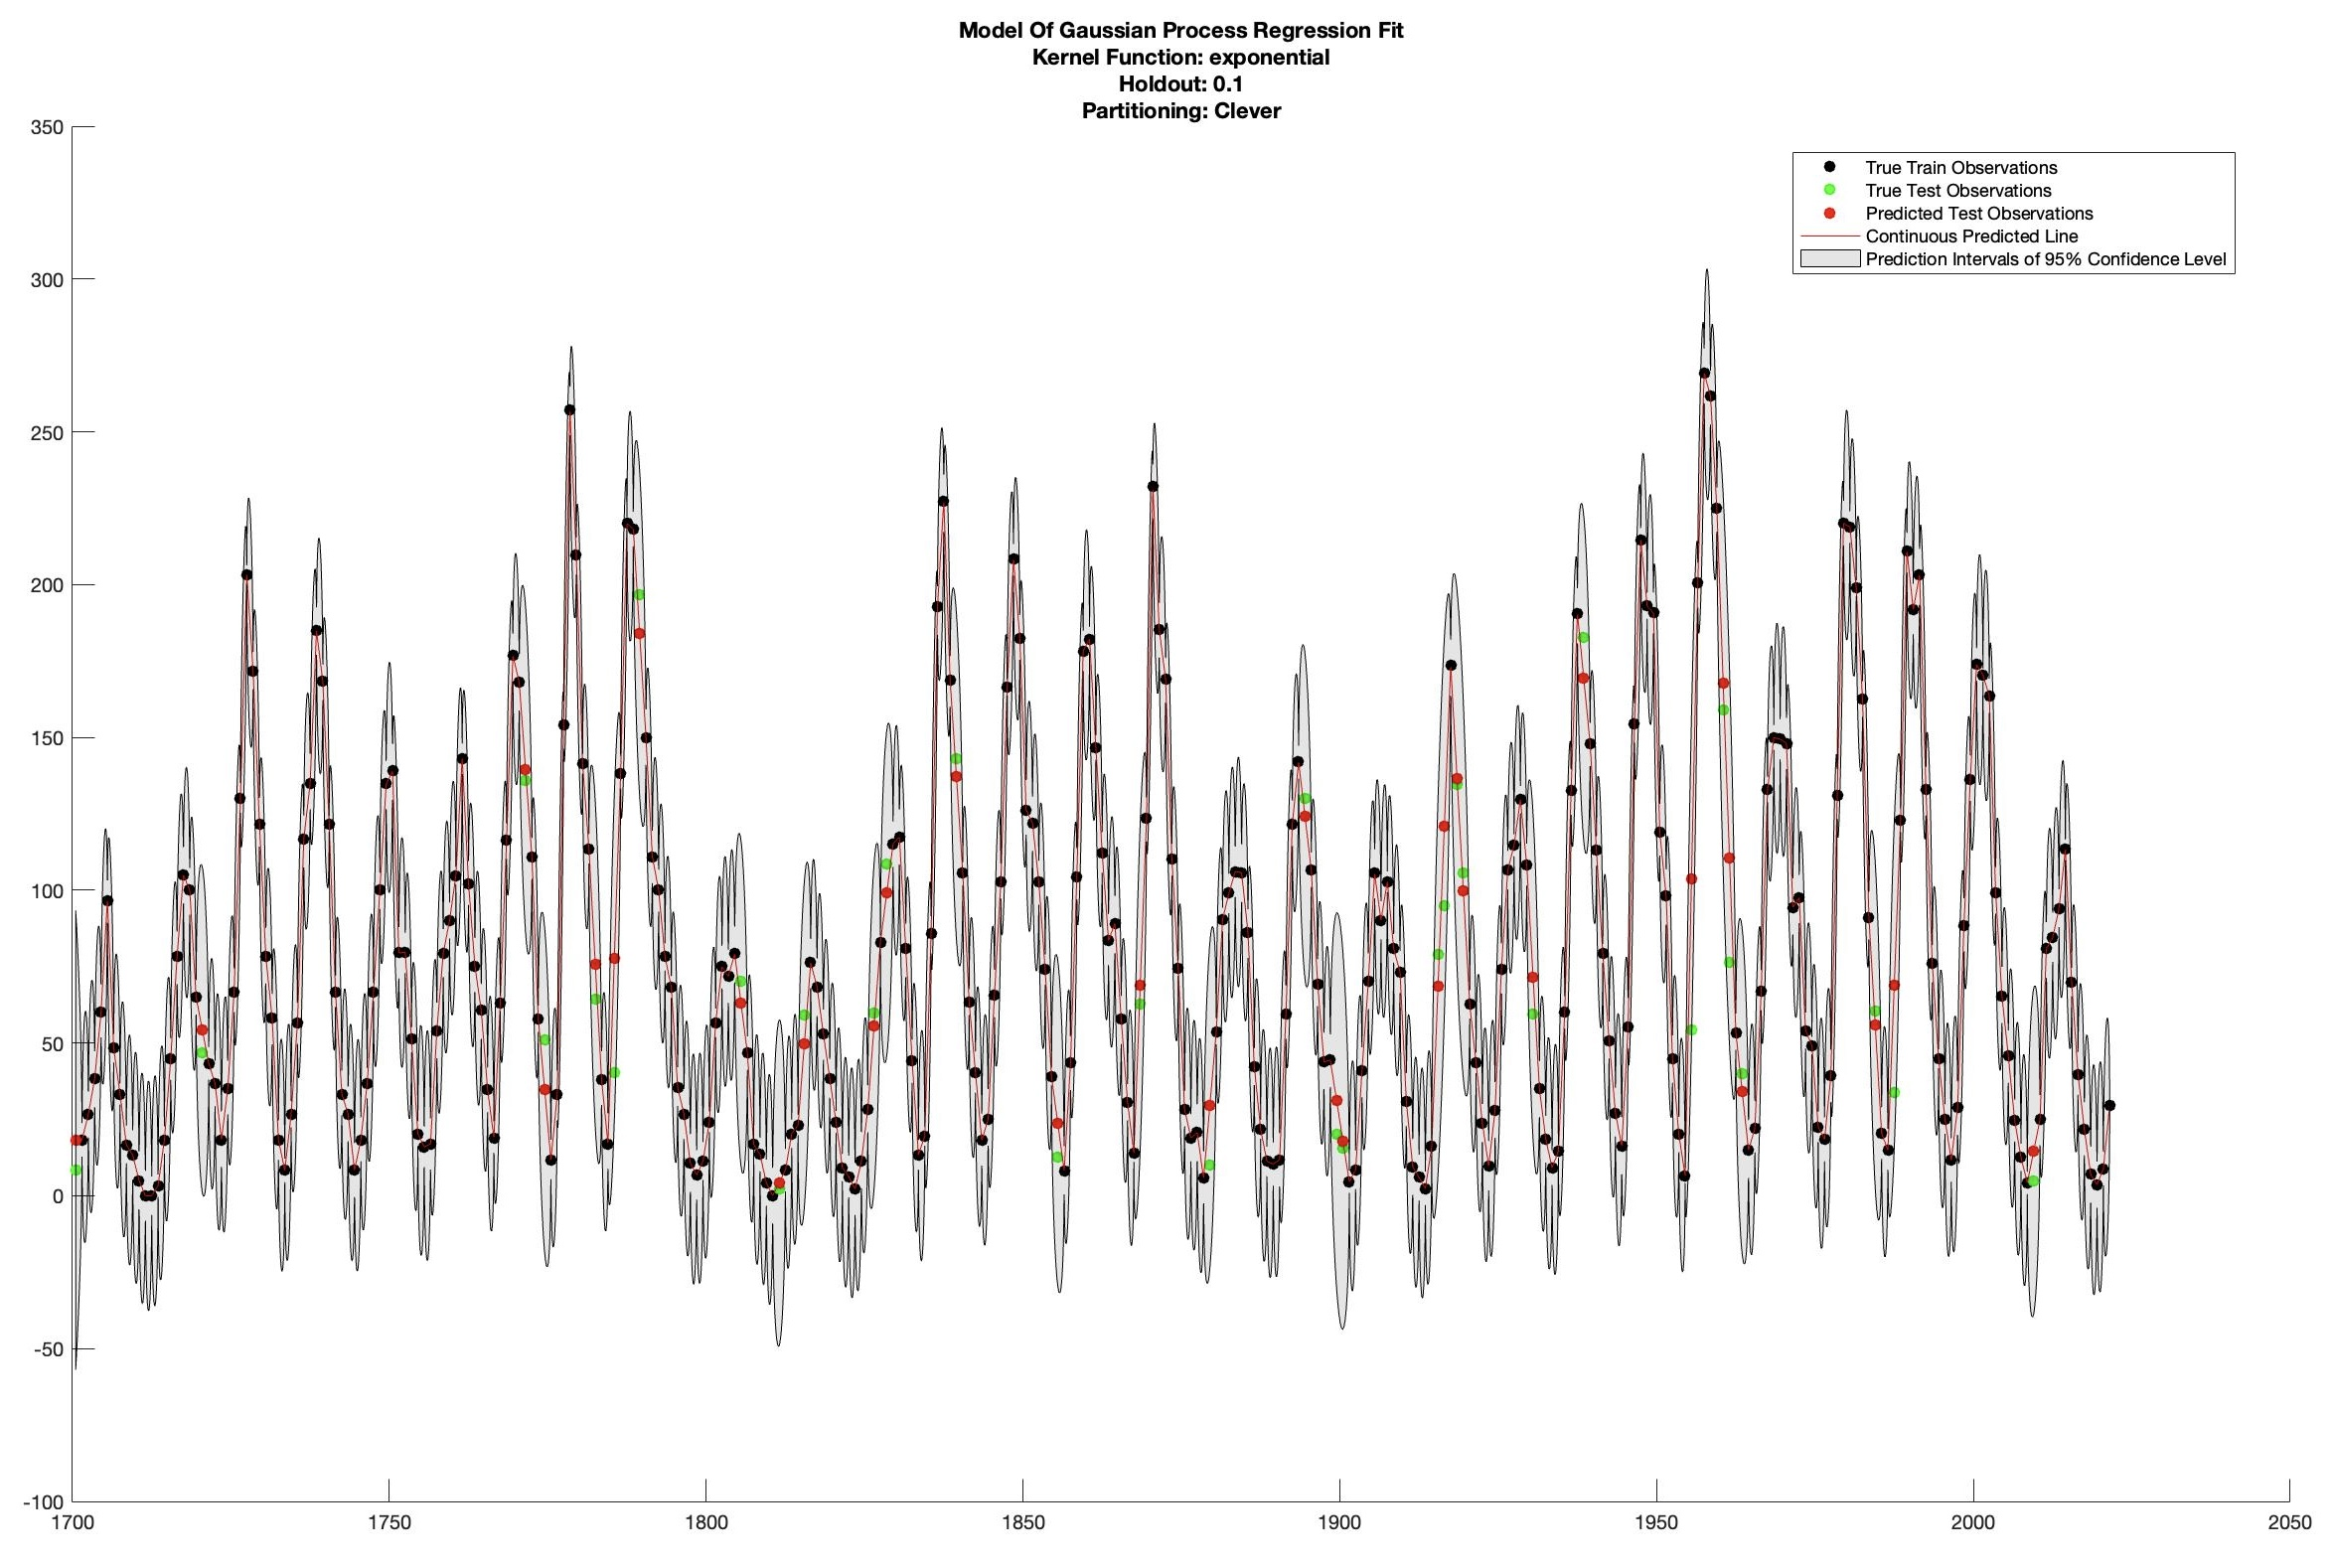
\includegraphics[scale = 0.2]{Exponential.jpg}
\end{figure}

\vspace{3cm}

\begin{figure}[H]
	\centering
	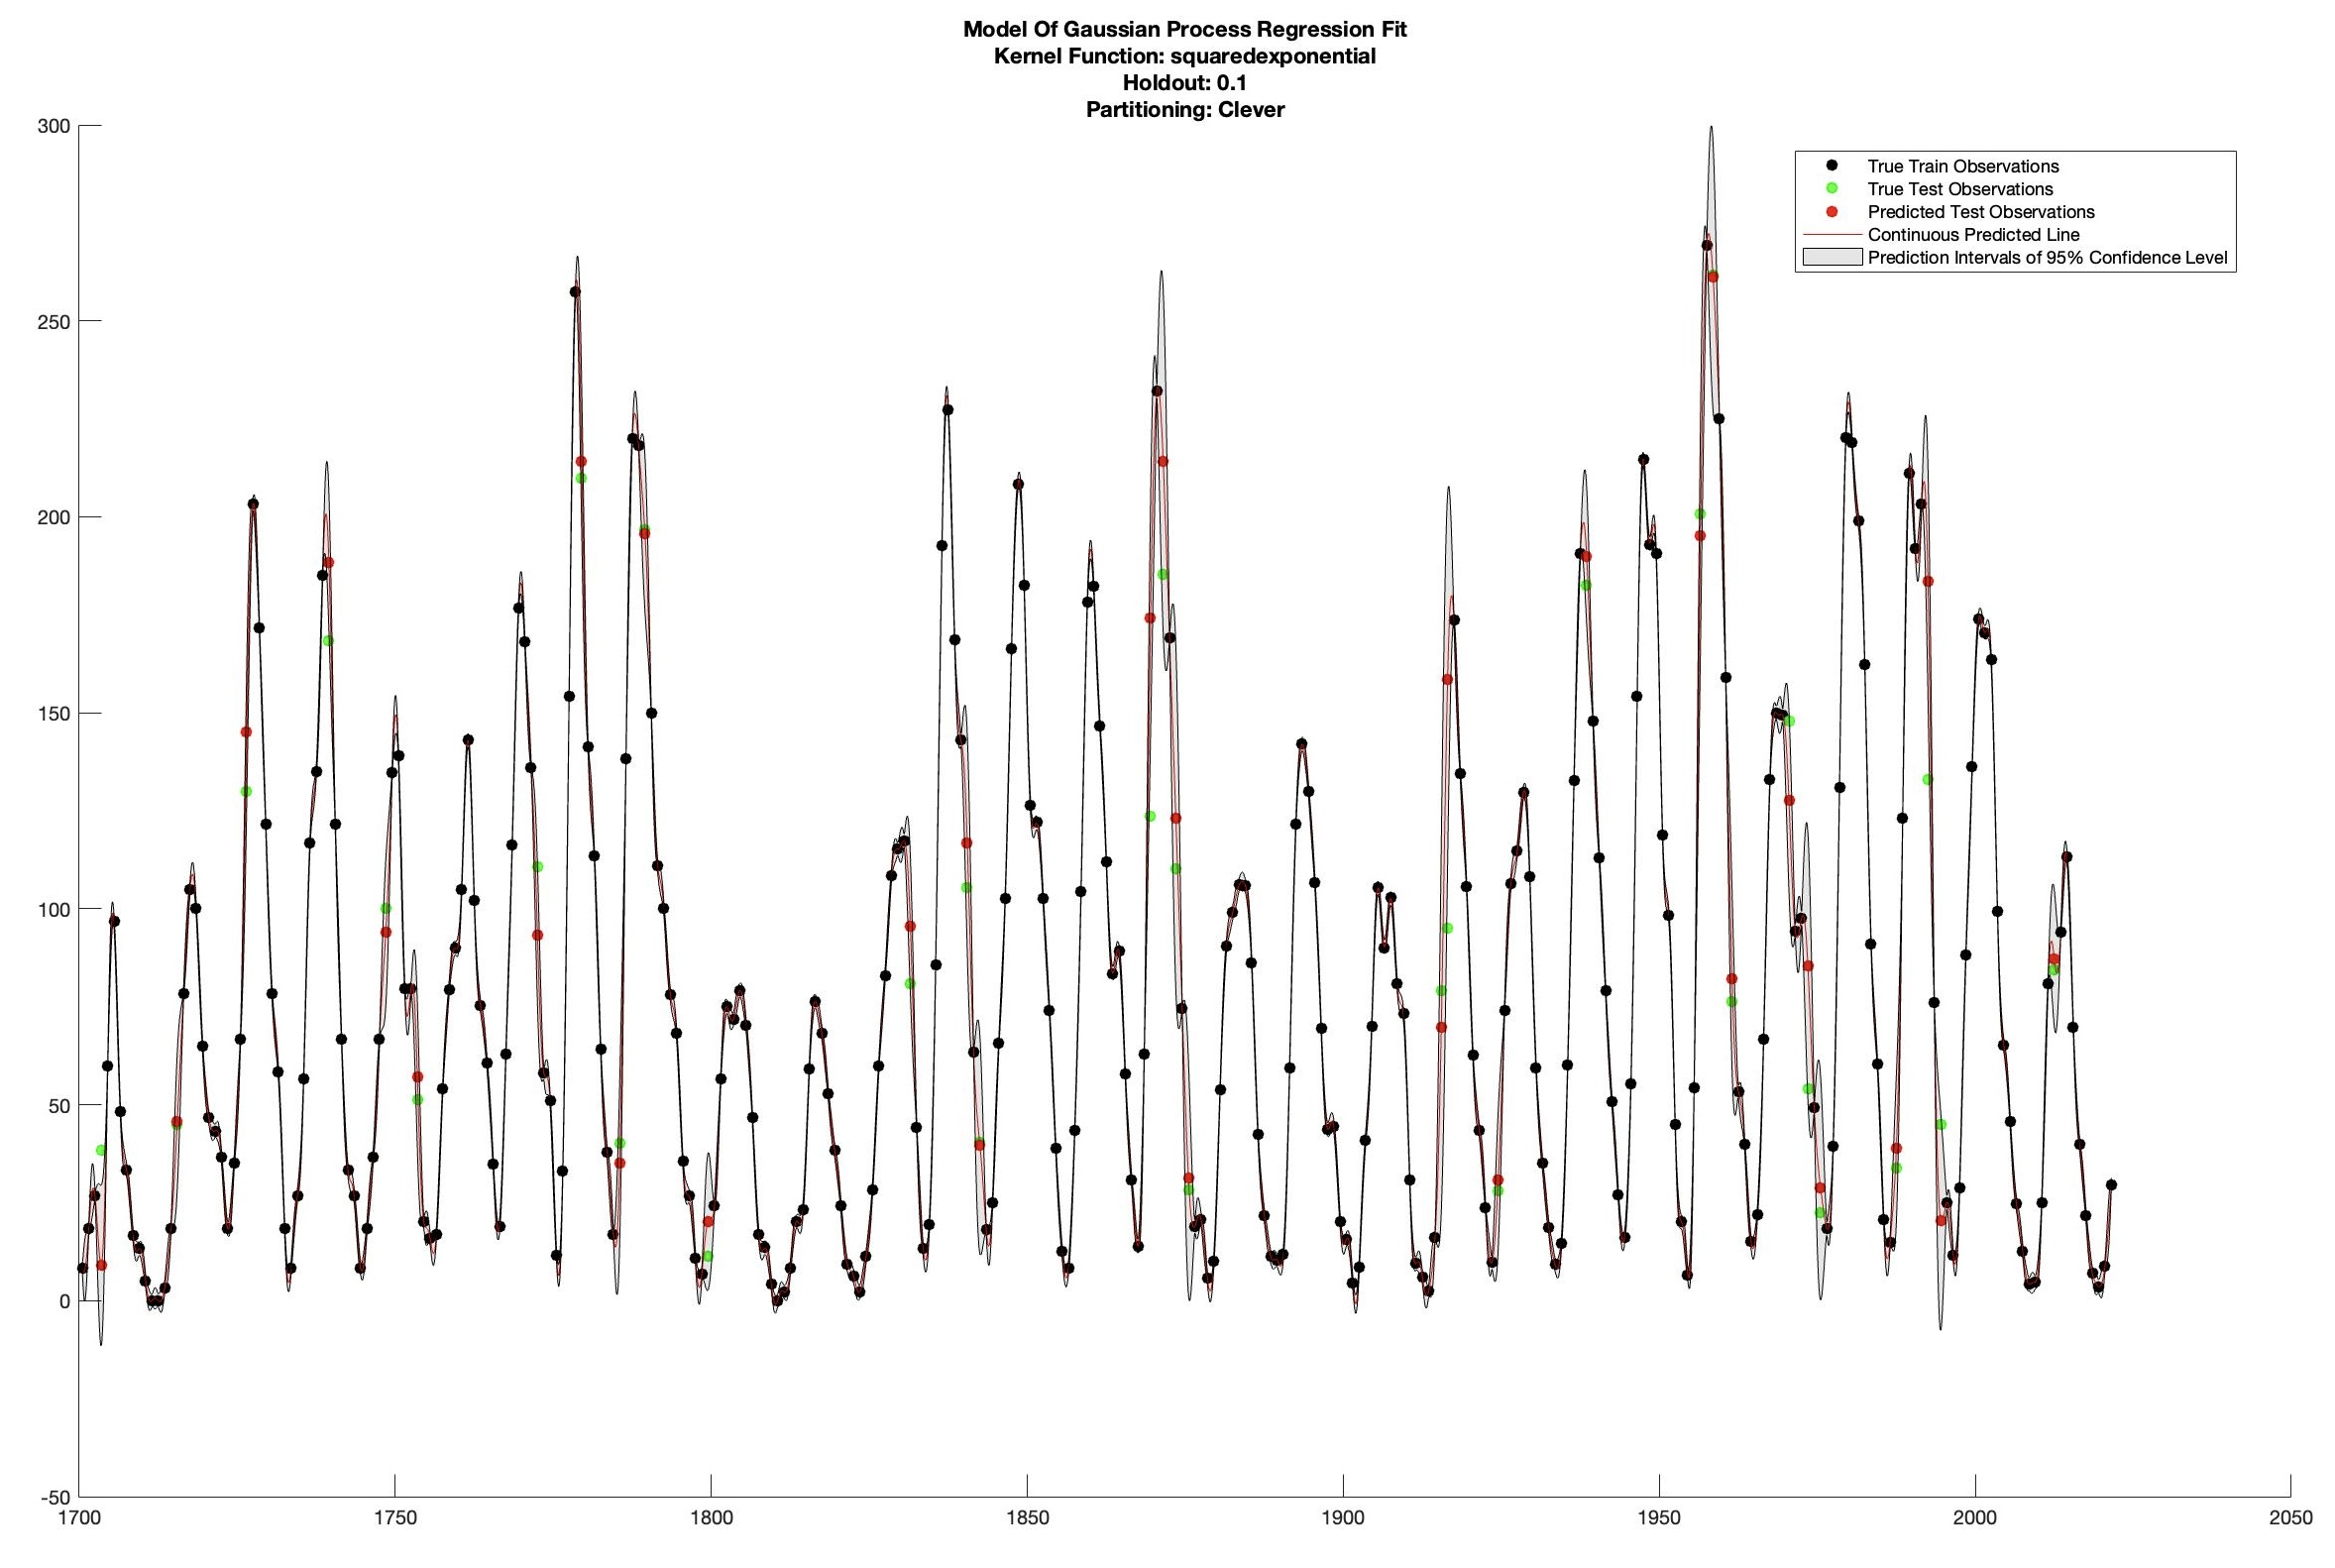
\includegraphics[scale = 0.2]{Squared_Exponential.jpg}
\end{figure}

\newpage

\begin{figure}[H]
	\centering
	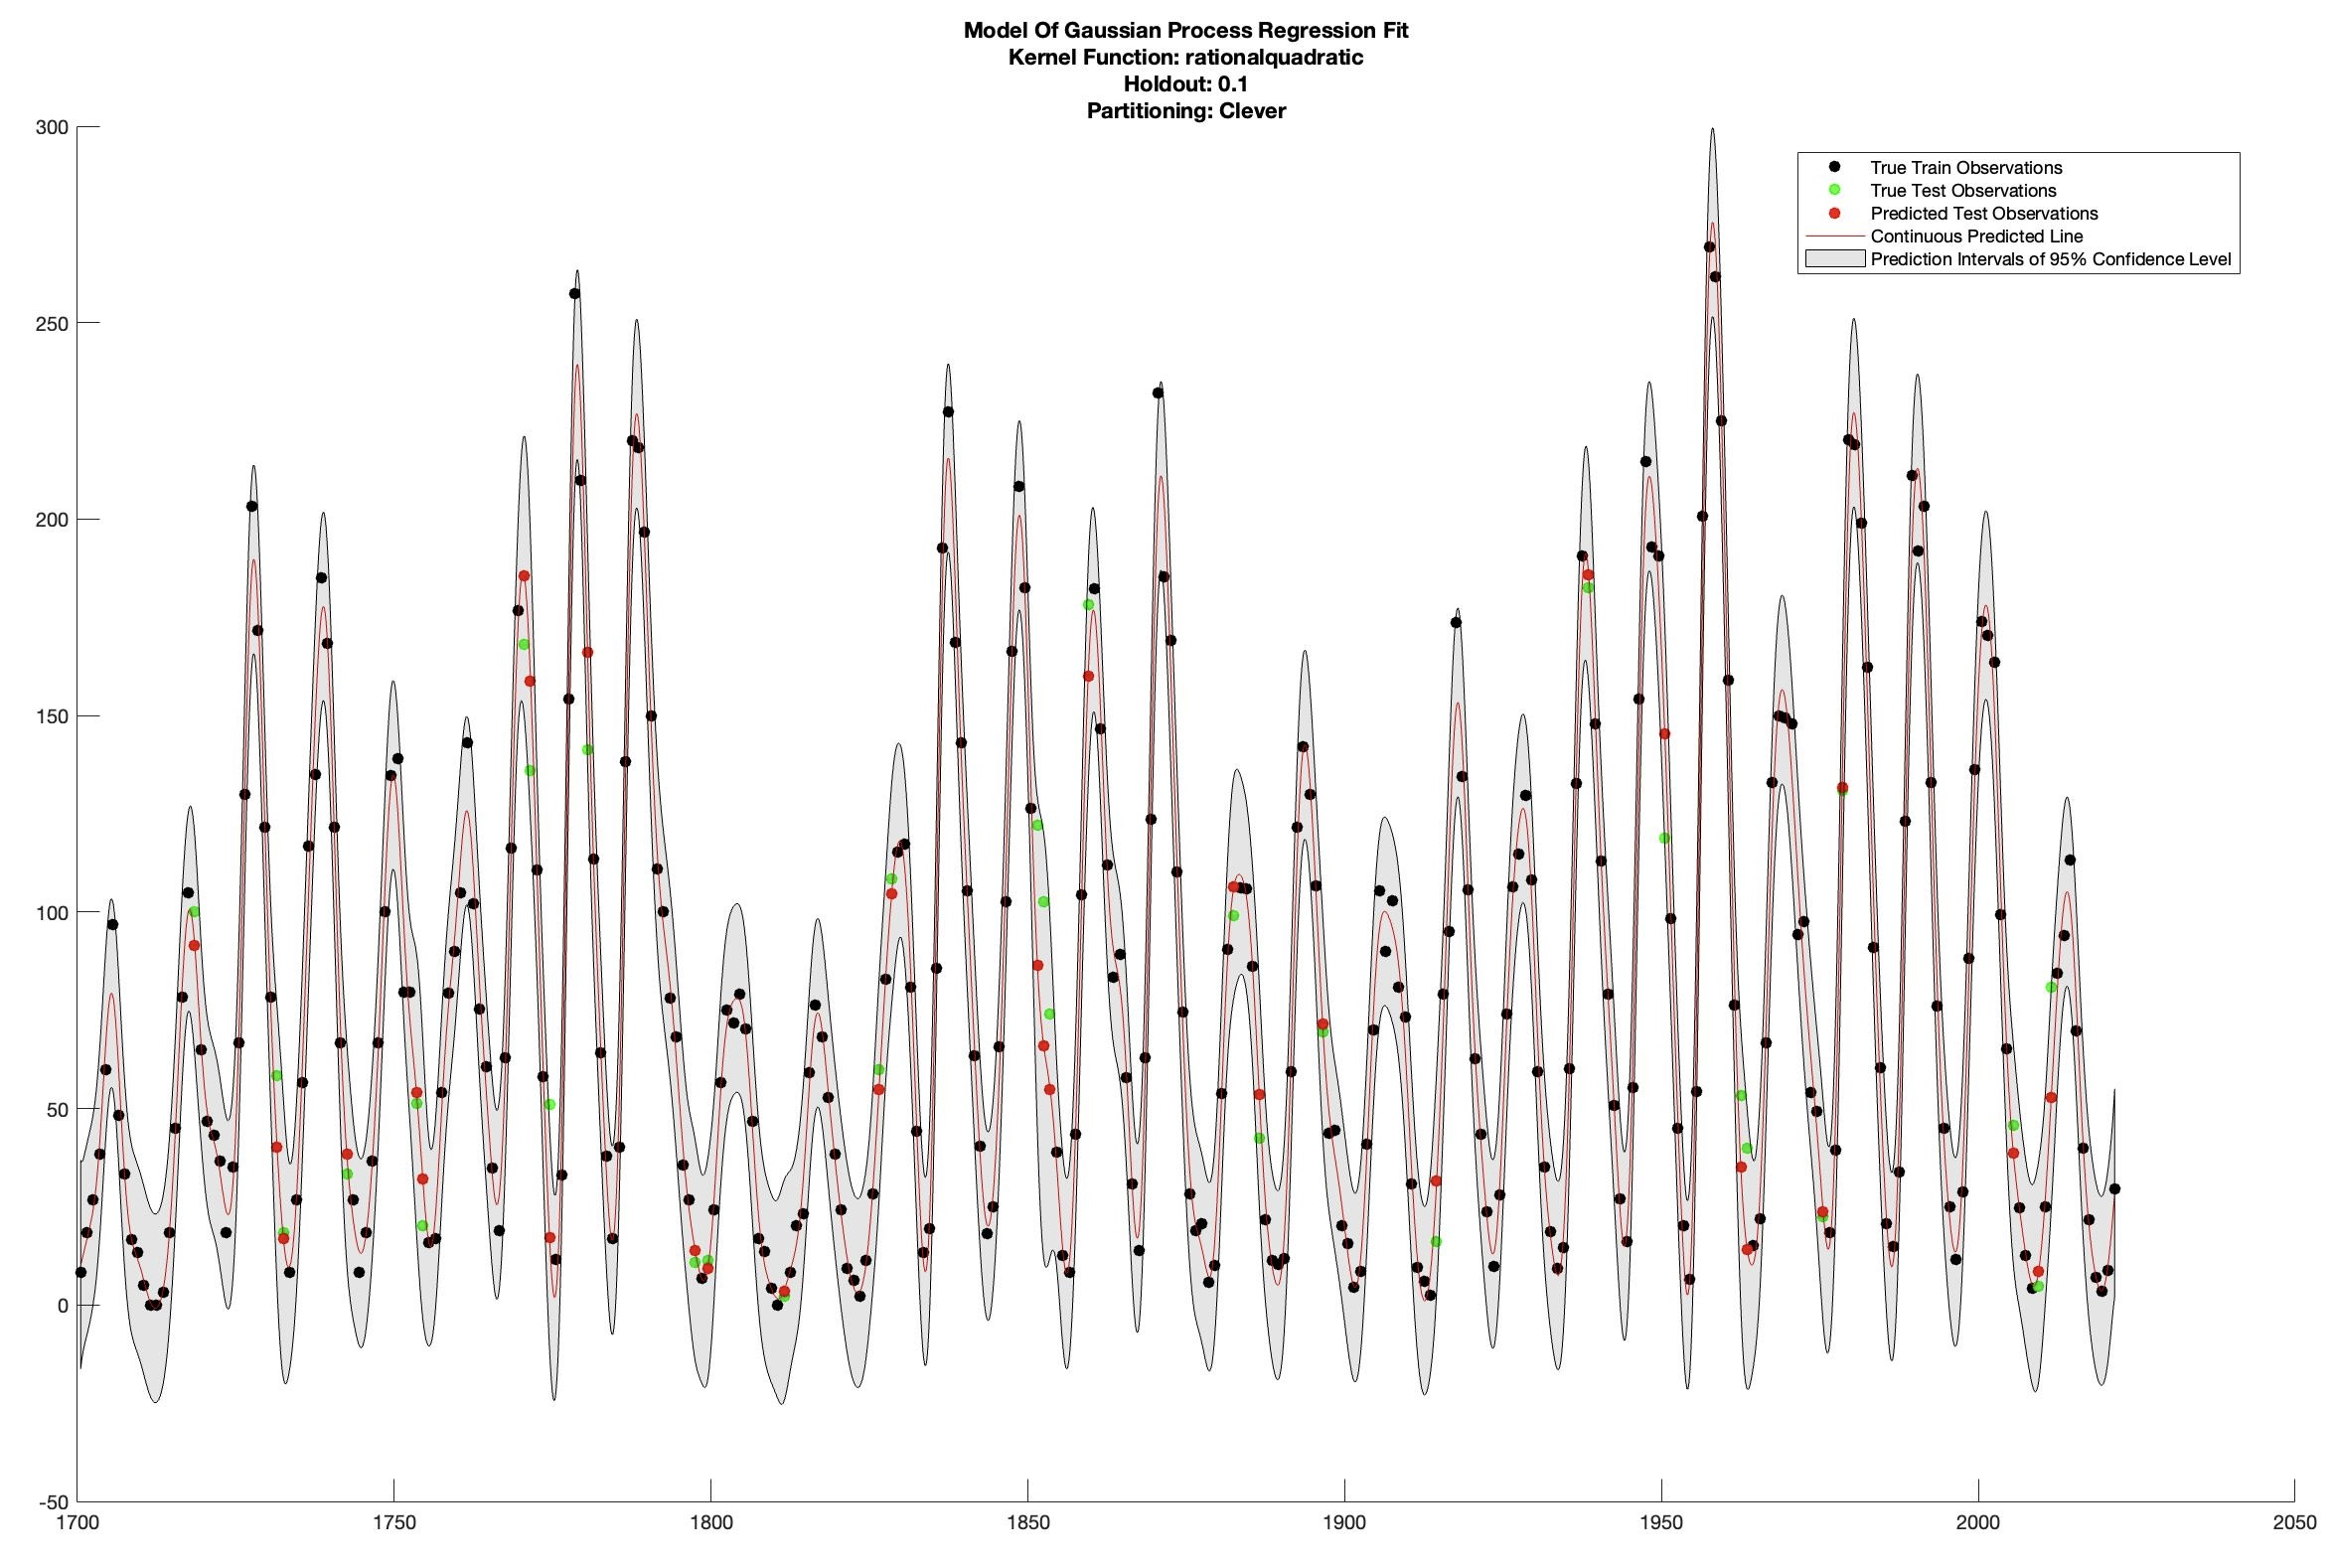
\includegraphics[scale = 0.2]{Rational_Quadratic.jpg}
\end{figure}

\vspace{3cm}

\begin{figure}[H]
	\centering
	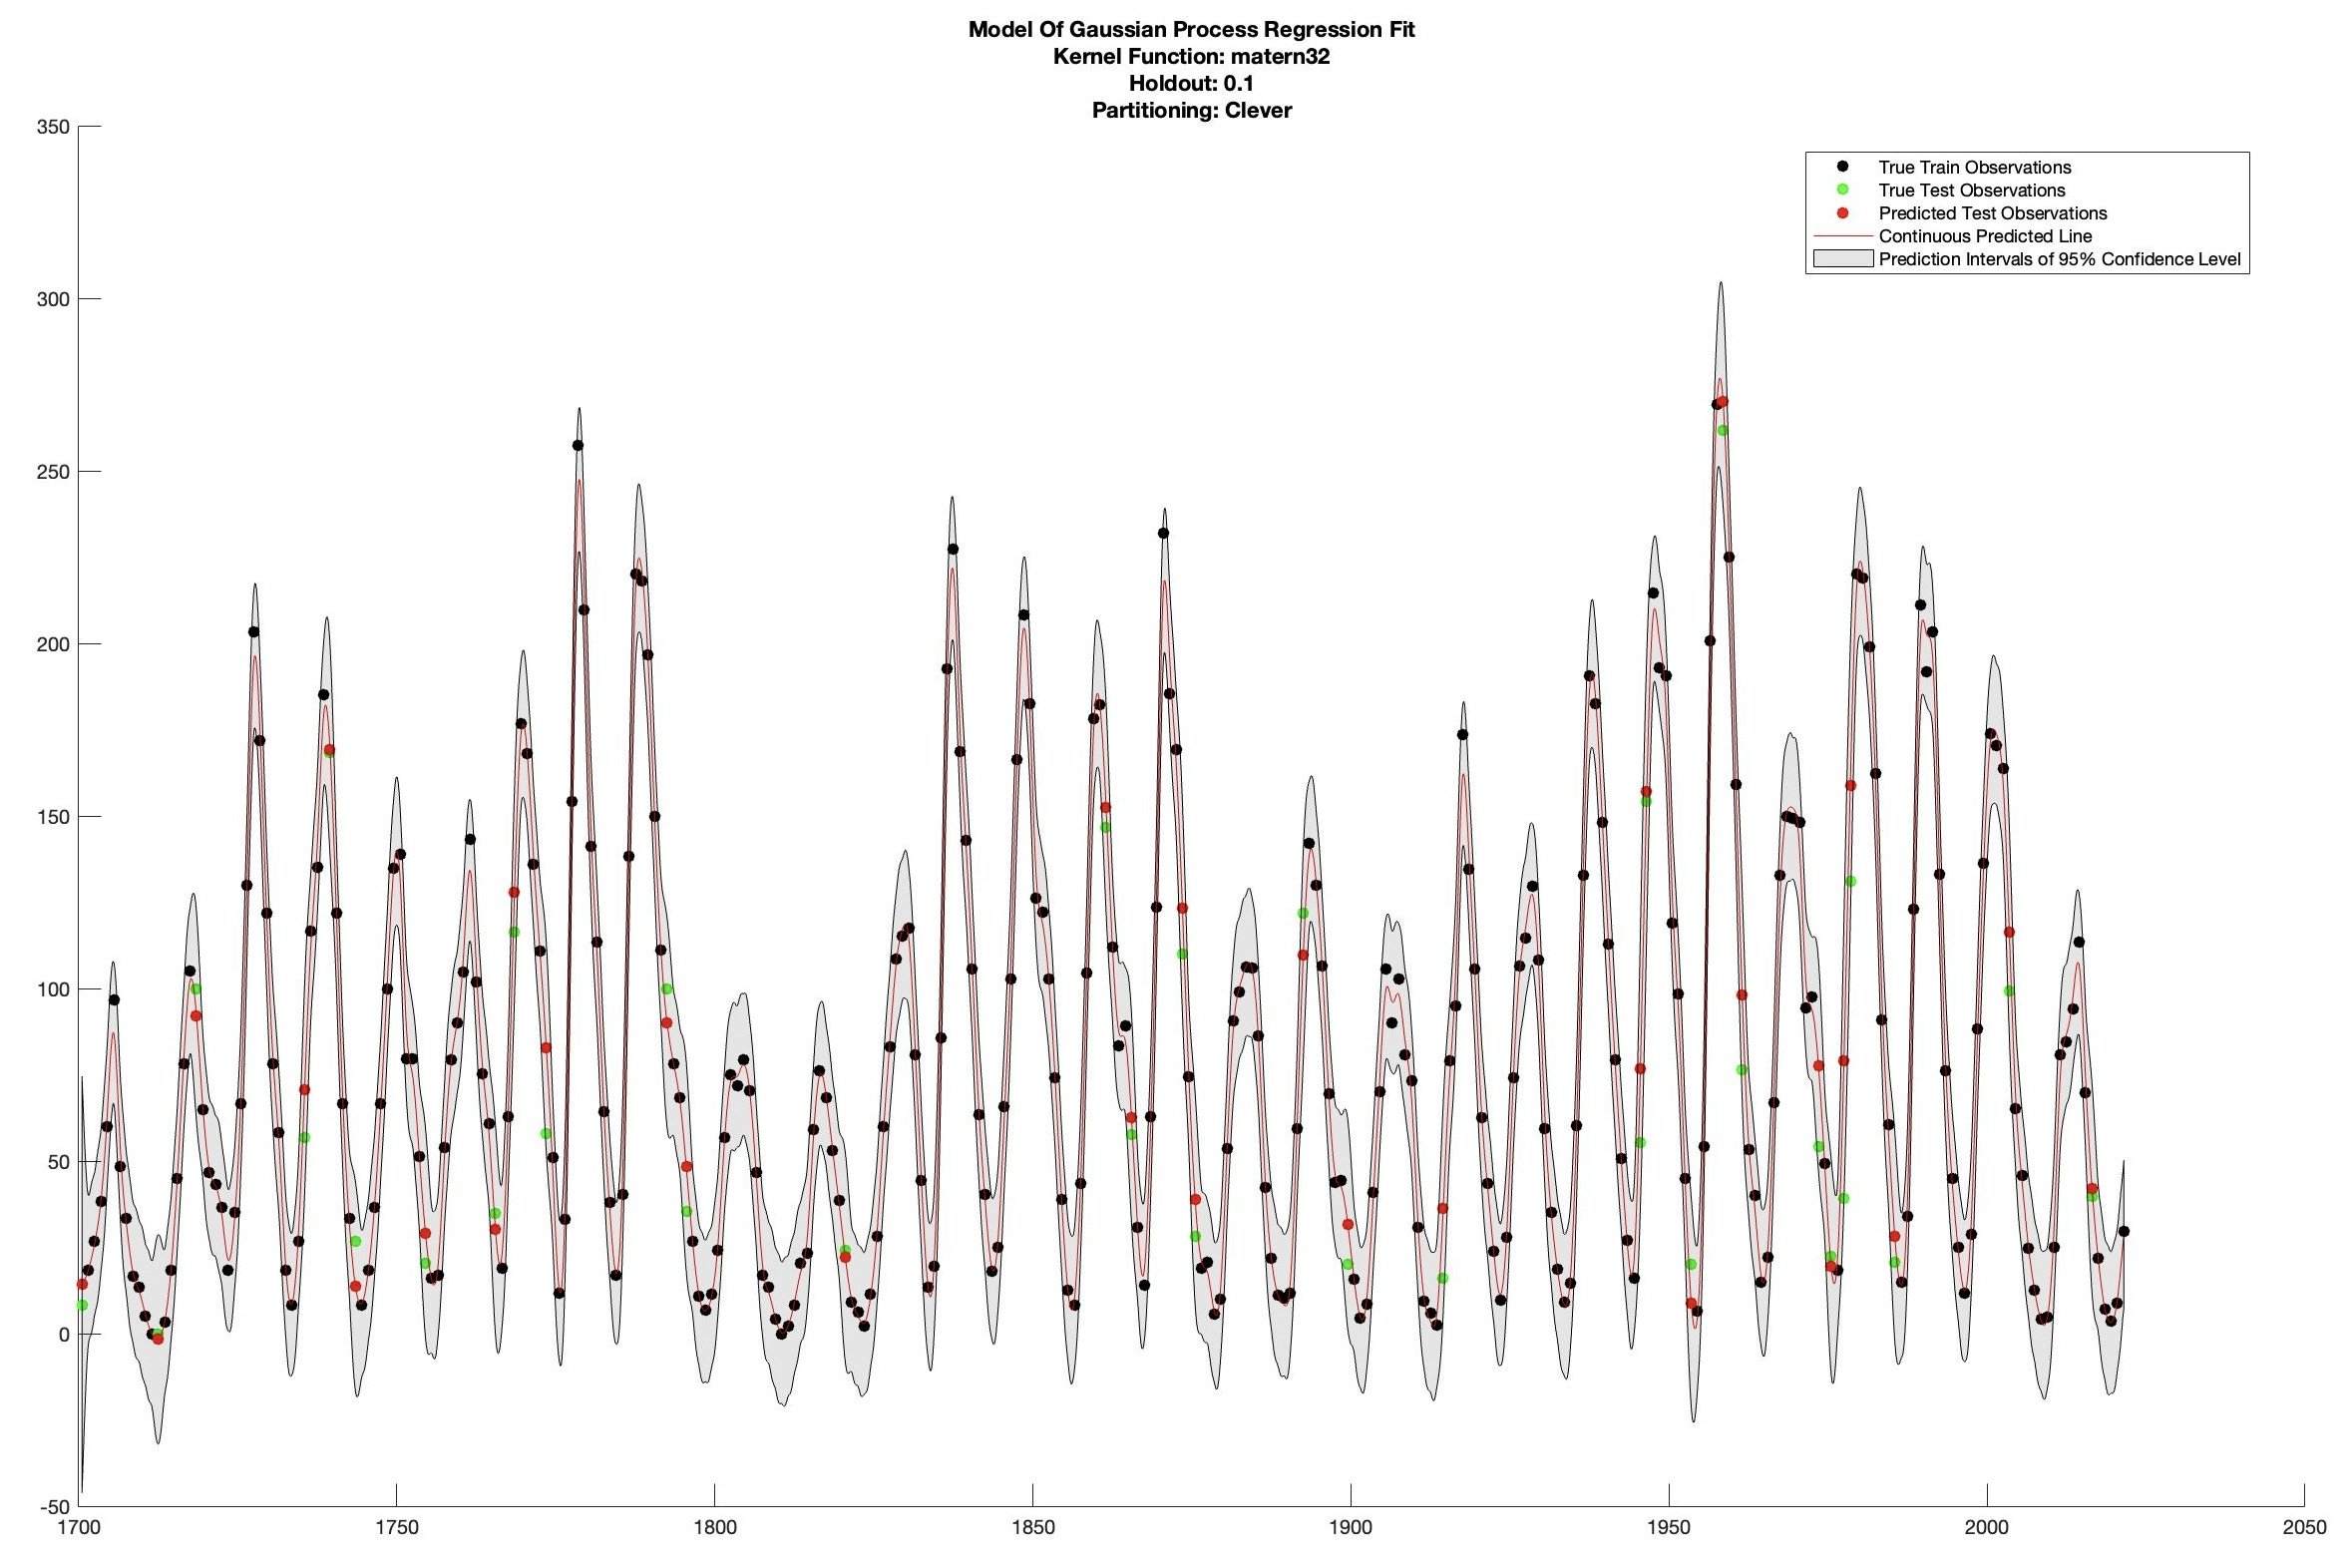
\includegraphics[scale = 0.2]{Matern32.jpg}
\end{figure}

\newpage

\begin{figure}[H]
	\centering
	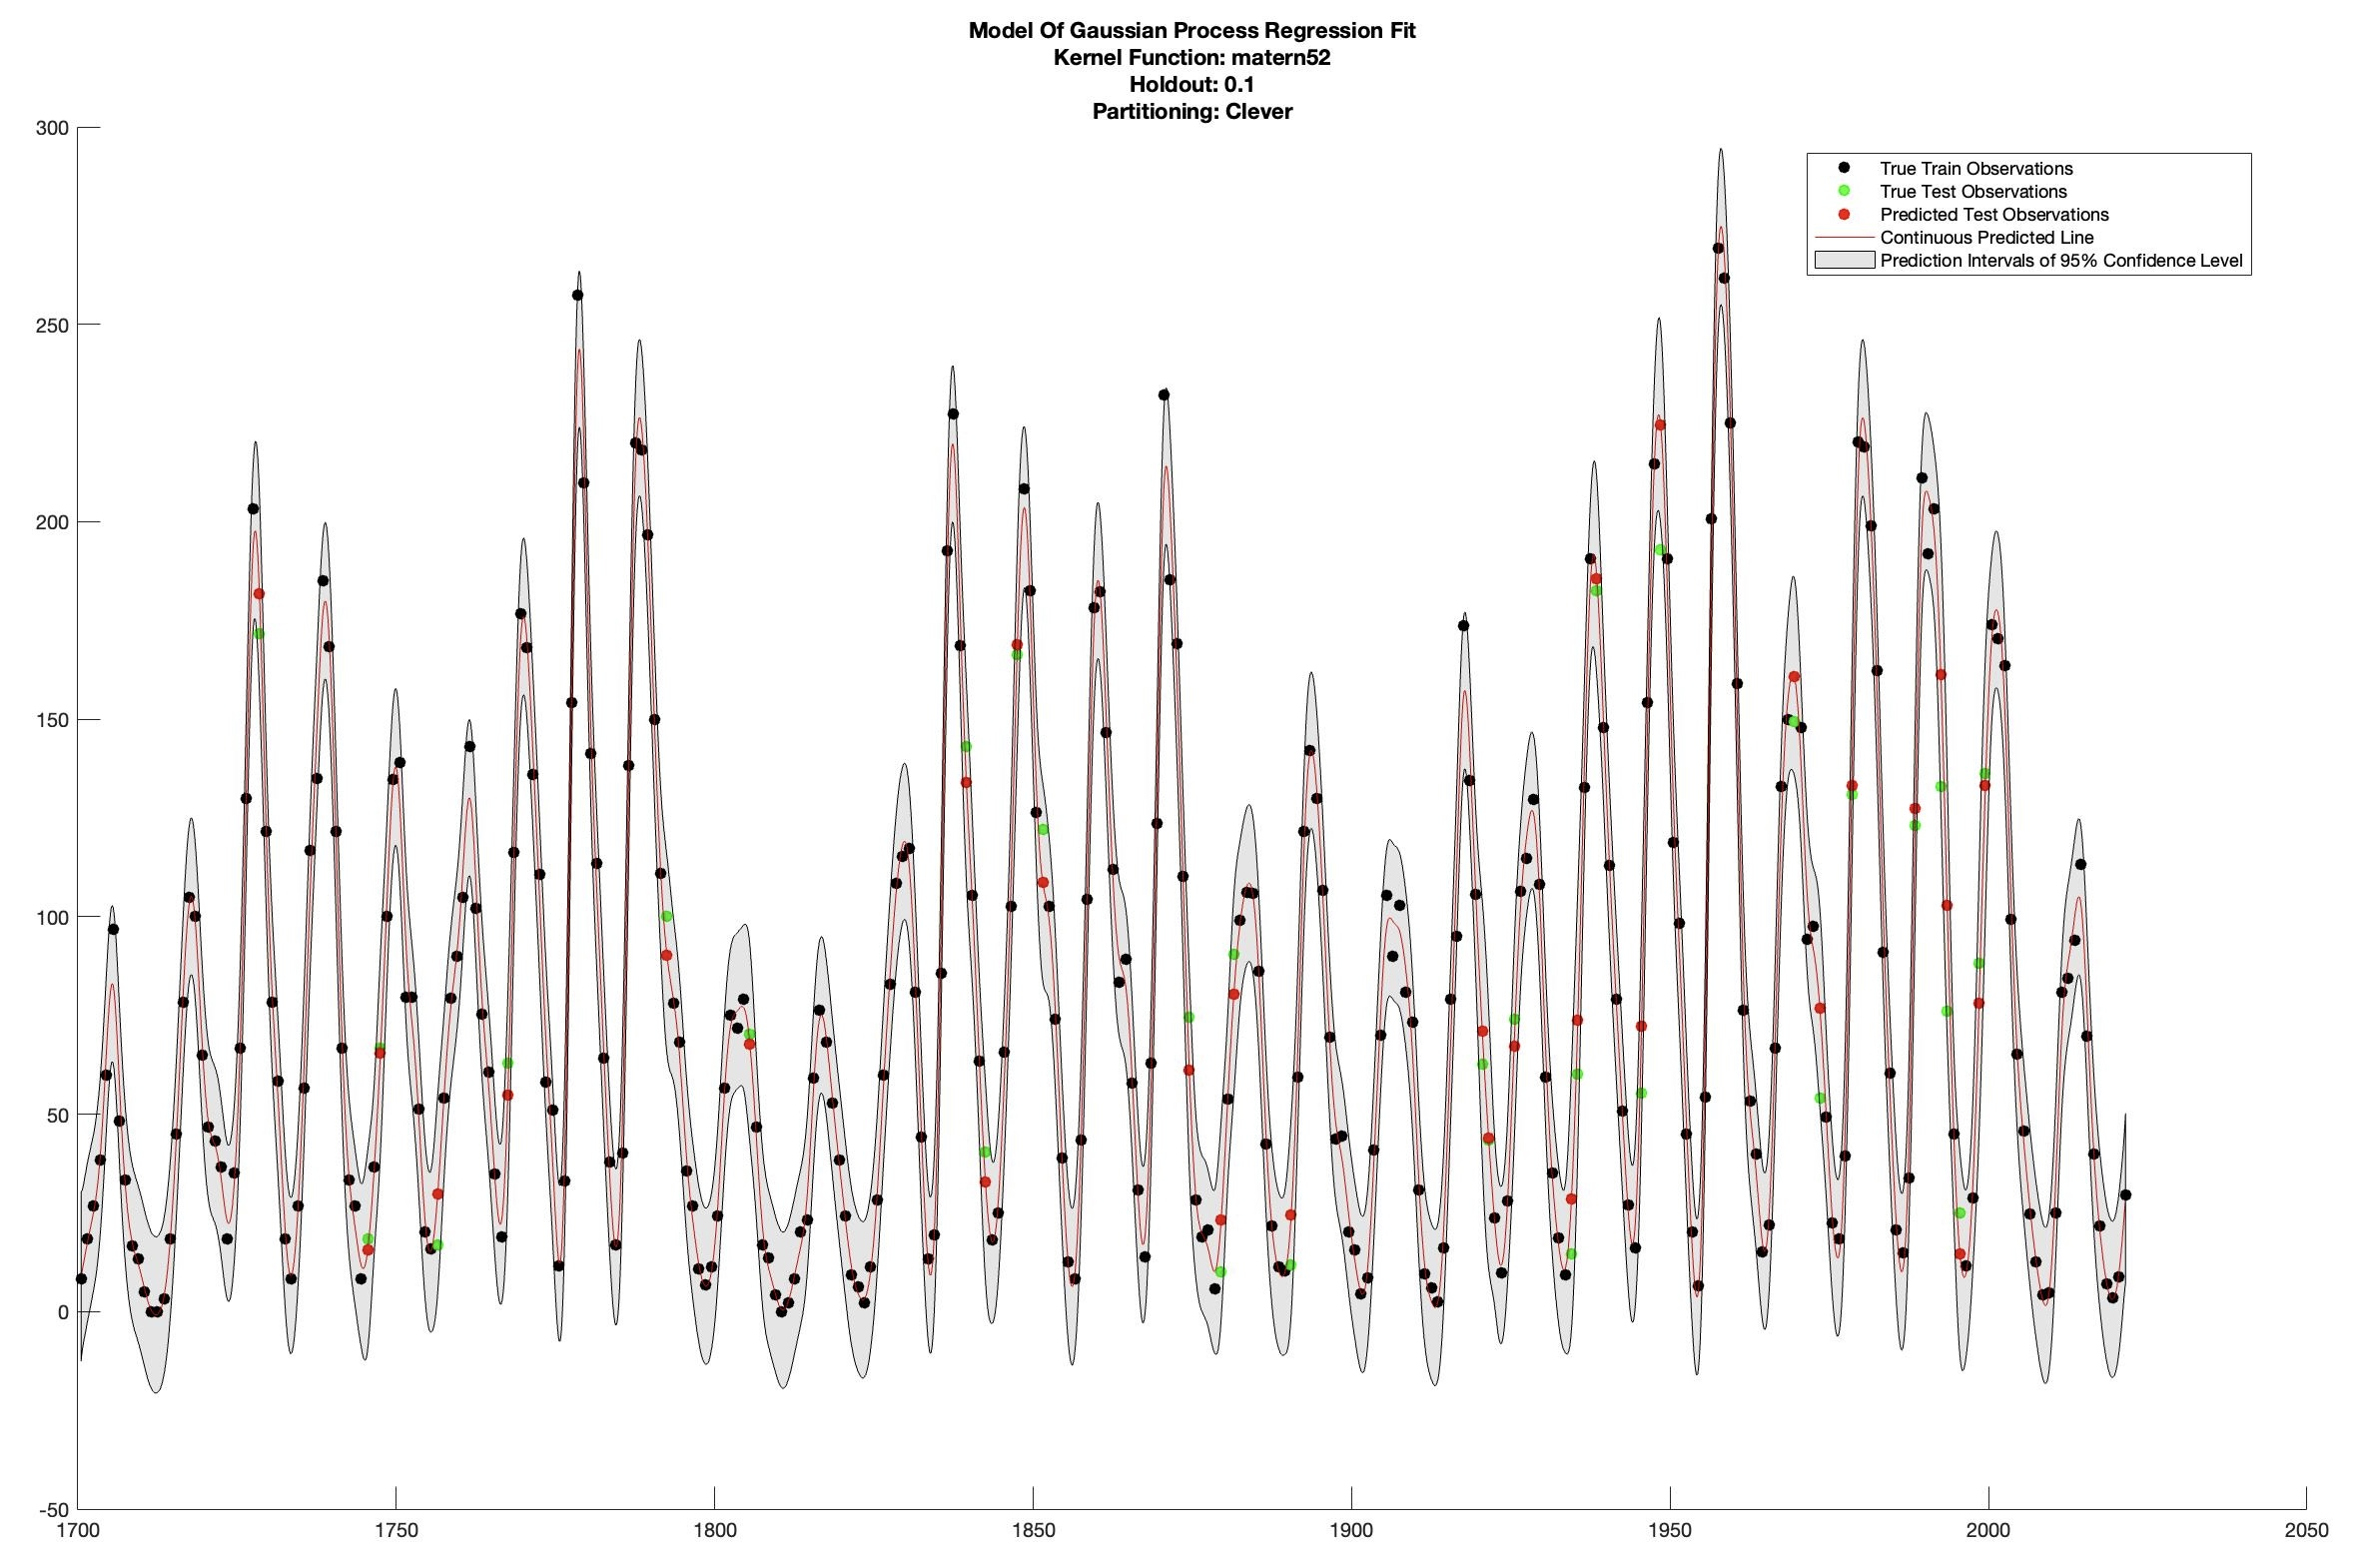
\includegraphics[scale = 0.2]{Matern52.jpg}
\end{figure}

\vspace{3cm}

\begin{figure}[H]
	\centering
	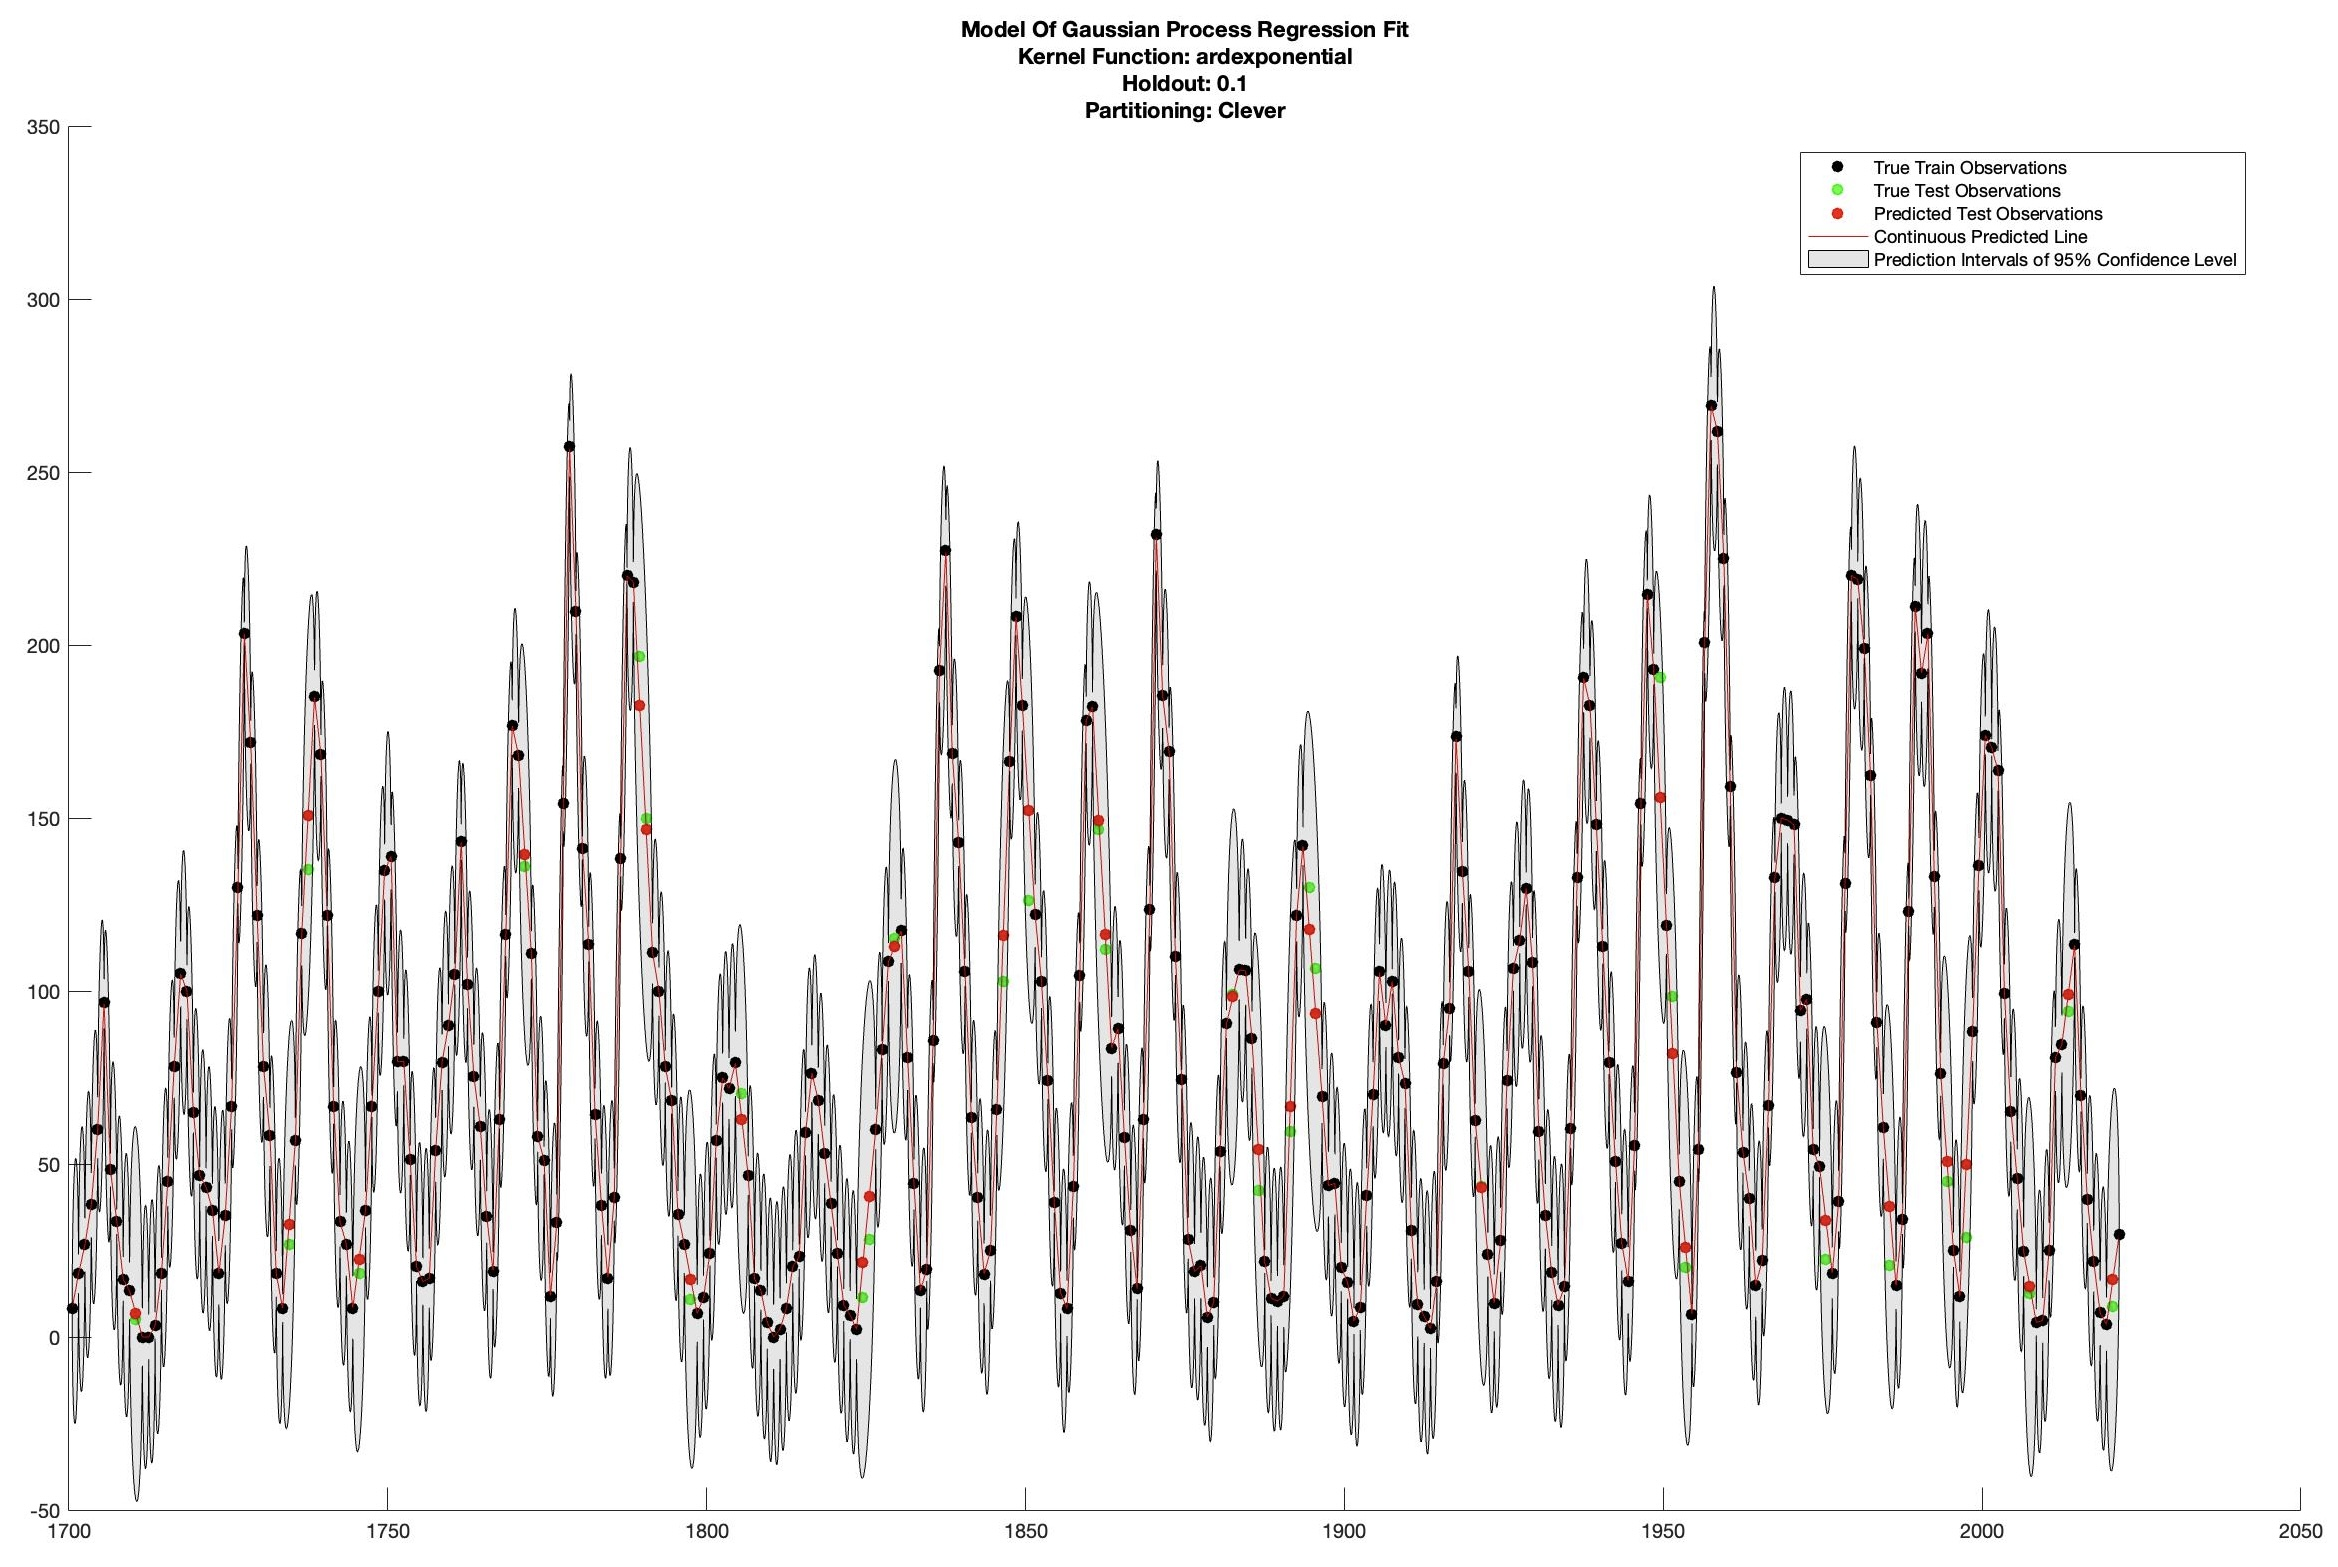
\includegraphics[scale = 0.2]{Ard_Exponential.jpg}
\end{figure}

\newpage

\begin{figure}[H]
	\centering
	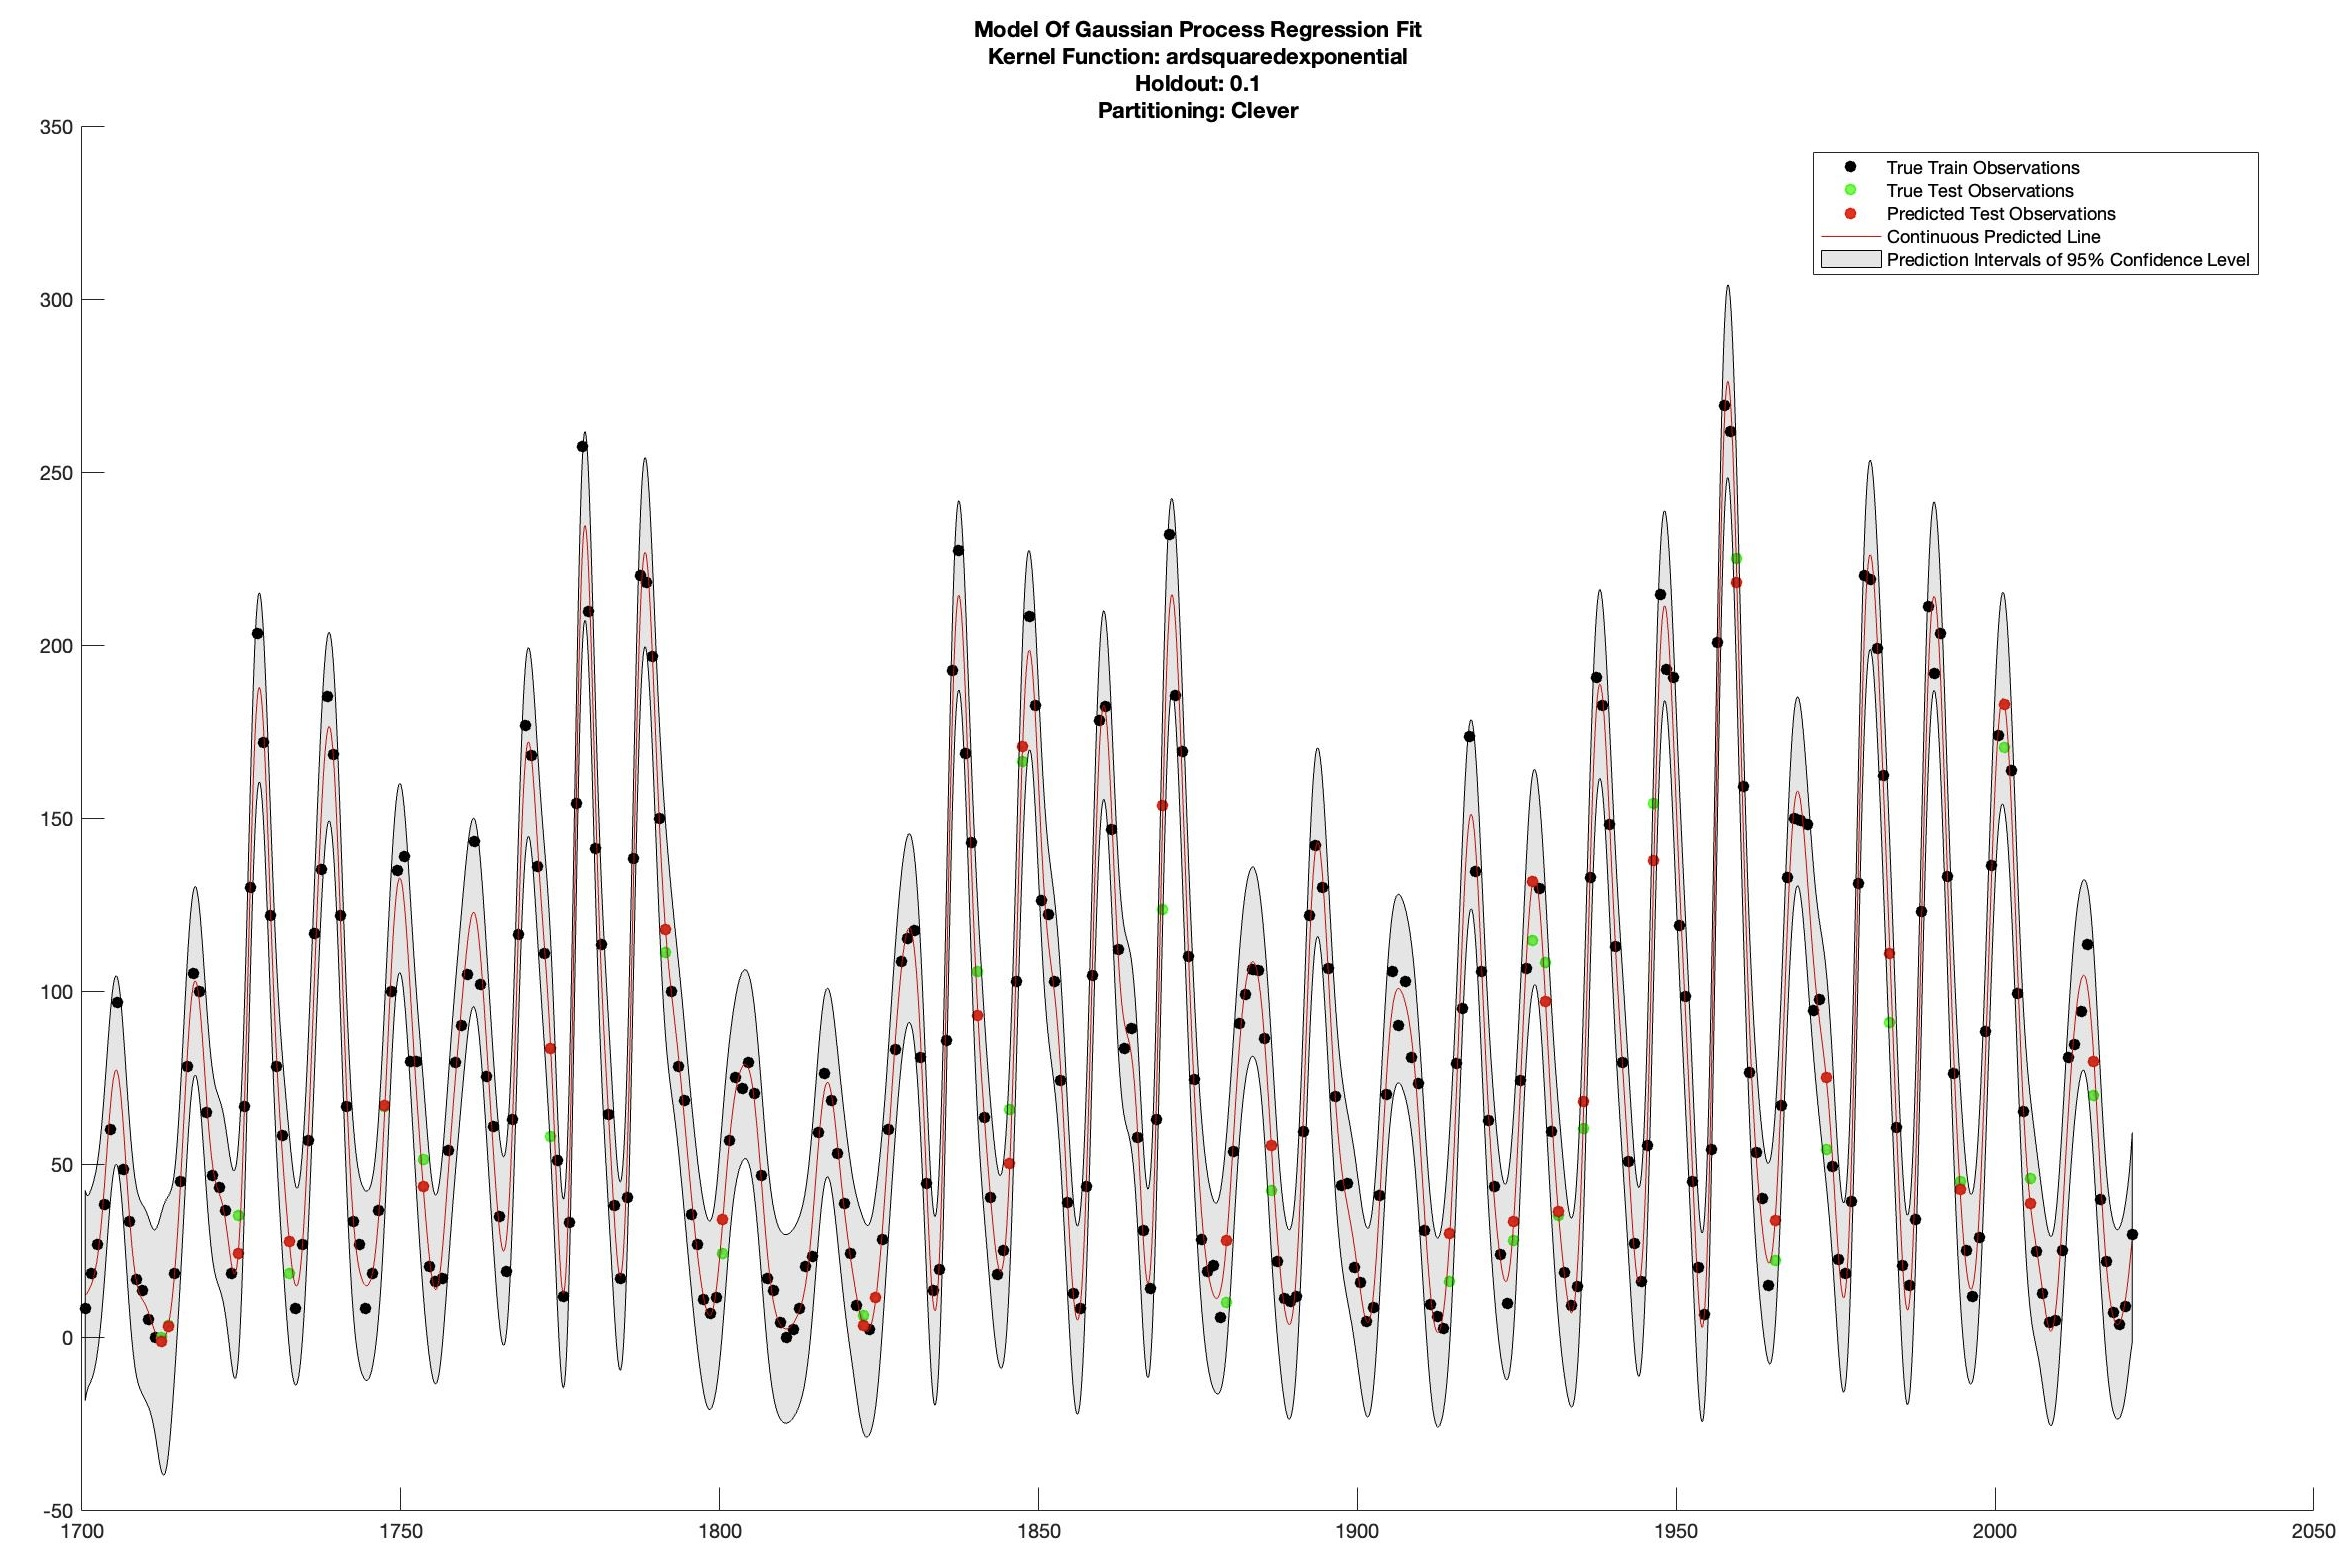
\includegraphics[scale = 0.2]{Ard_Squared_Exponential.jpg}
\end{figure}

\vspace{3cm}

\begin{figure}[H]
	\centering
	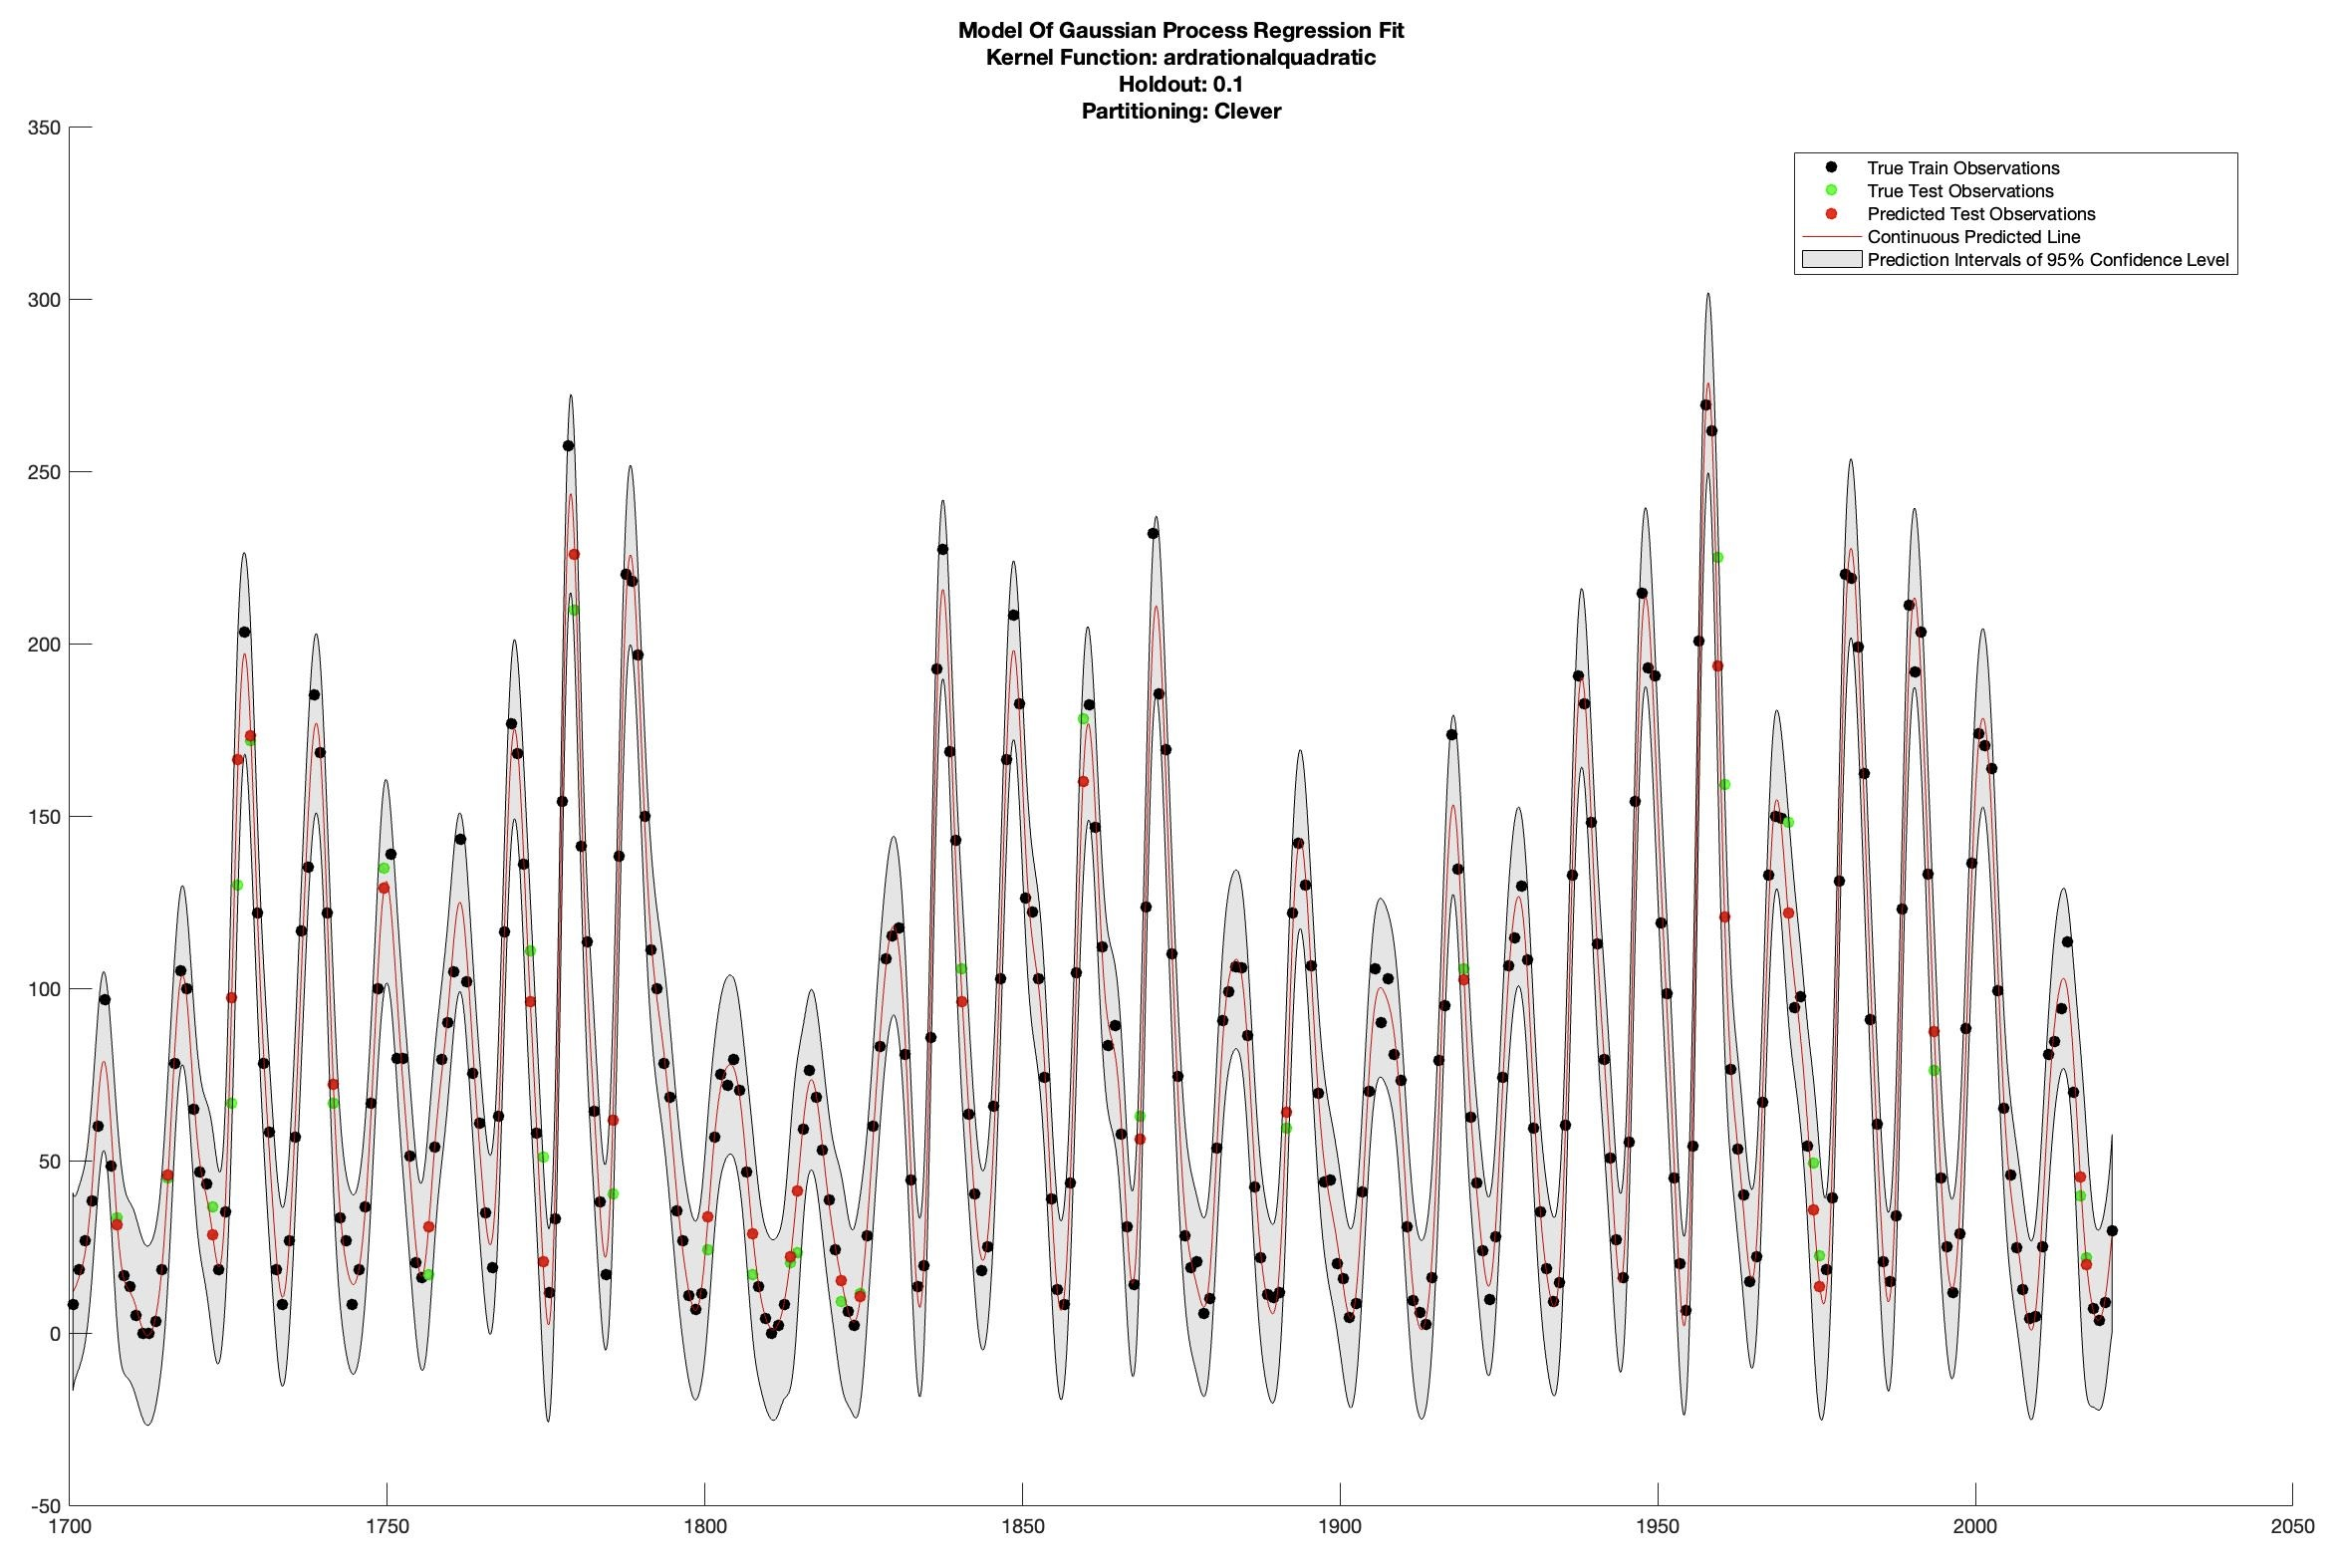
\includegraphics[scale = 0.2]{Ard_Rational_Quadratic.jpg}
\end{figure}

\newpage

\begin{figure}[H]
	\centering
	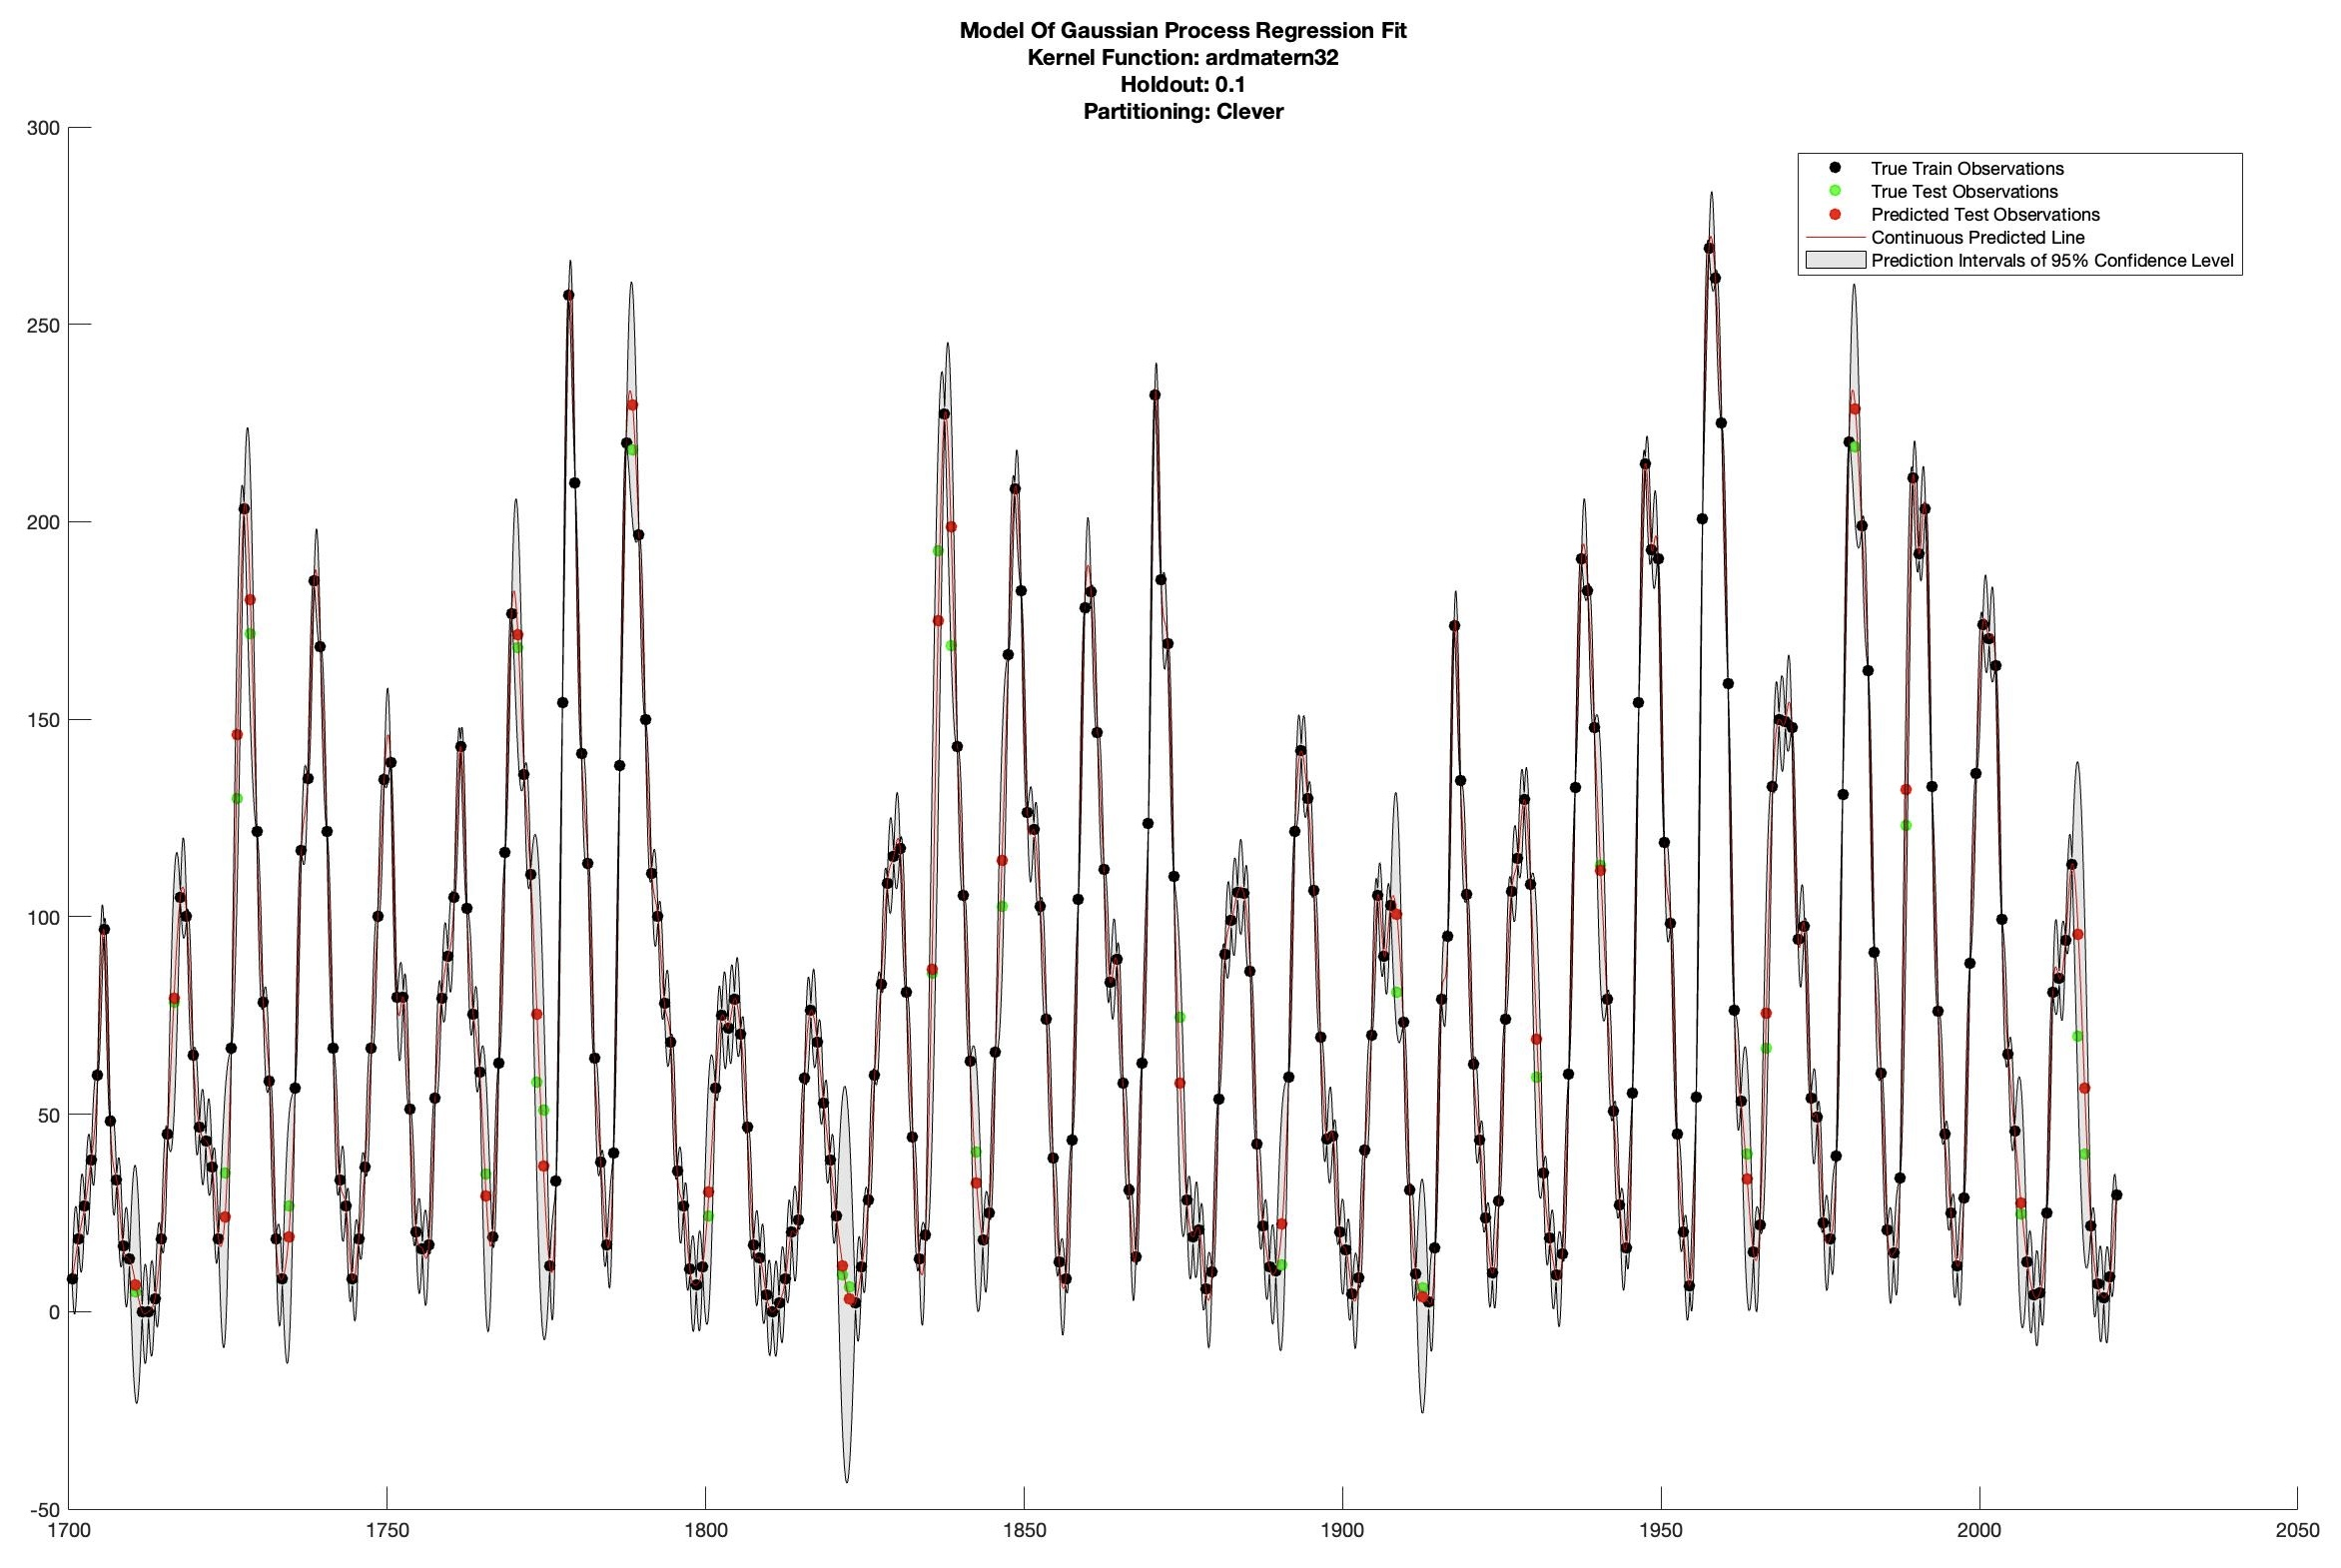
\includegraphics[scale = 0.2]{Ard_Matern32.jpg}
\end{figure}

\vspace{3cm}

\begin{figure}[H]
	\centering
	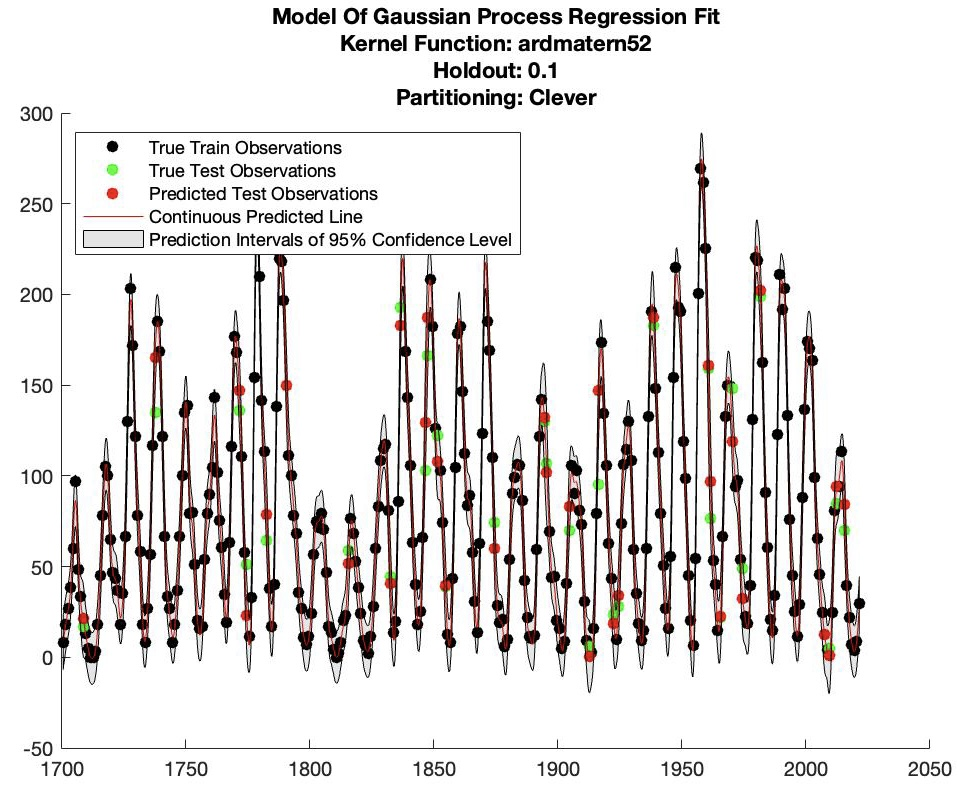
\includegraphics[scale = 0.5]{Ard_Matern52.jpg}
\end{figure}

\newpage

\sectionmark{}
\noindent
\boldmark{\Large{{\color{crimsonglory}CONCLUSION}}}

\normalsize
\noindent
Overall, we are in position to realize the importance of using Gaussian Process Regression as a tool for curve fitting and training a model that is capable of making accurate predictions. Such a model gives us at the same time uncertainty information about each prediction, unlike other non-probabilistic methods. For that purpose, an important part, before training, is to determine the kernel function and tune its hyperparameters. As we said, an approach is to maximize the log marginal likelihood. The partition of the data into train and test subsets plays a significant role to the training. An intelligent selection of the train set, in a way that it includes turning points (peaks), gives way better performance of the GPR model. In our case of sunspots data-set, we conclude that a pretty good model is the one with ``Ard Matern 3/2" kernel function, because it gives very small RRMSE and strict prediction intervals of $95\%$ confidence level. Finally, normalization of the original data-set is not preferred and, as for the hyperparameter tuning, Bayesian optimization is being used.

%\vspace{2cm}

%\sectionmark{}
%\noindent
%\boldmark{\Large{{\color{crimsonglory}RECOMMENDATIONS}}}

%\noindent
%In this

\vspace{2cm}

\sectionmark{}
\noindent
\boldmark{\Large{{\color{crimsonglory}REFERENCES}}}

\normalsize
\noindent
Some useful references and documentations are the following (clickable):
\begin{itemize}
    \item \href{https://www.mathworks.com/help/stats/gaussian-process-regression-models.html}{Gaussian Process Regression Models (Matlab documentation)}
    \item \href{https://www.mathworks.com/help/stats/kernel-covariance-function-options.html}{Kernel (Covariance) Function Options (Matlab documentation)}
    \item \href{https://www.mathworks.com/help/stats/fitrgp.html}{Matlab function {\color{blue}fitrgp($\cdot$)} documentation}
    \item \href{https://www.mathworks.com/help/stats/compactregressiongp.predict.html}{Matlab function {\color{blue}predict($\cdot$)} documentation}
    \item \href{https://www.mathworks.com/help/stats/compactregressiongp.loss.html}{Matlab function {\color{blue}loss($\cdot$)} documentation}
    \item \href{https://www.mathworks.com/help/stats/cvpartition.html}{Matlab function {\color{blue}cvpartition($\cdot$)} documentation}
    \item Roberts S., Osborne M., Ebden M., Reece S., Gibson N. and Aigrain S. (2013). Gaussian processes for time-series modelling. Philosophical Transactions of the Royal Society.\\ \url{https://doi.org/10.1098/rsta.2011.0550}
    \item Jie Wang (2022). An Intuitive Tutorial to Gaussian Processes Regression. Ingenuity Labs Research Institute, Queen’s University, 69 Union St W, Kingston, K7L 3N6, ON, Canada. \url{
https://doi.org/10.48550/arXiv.2009.10862}
    \item Lindholm, Andreas and Wahlstr\"om, Niklas and Lindsten, Fredrik and Sch\"on, Thomas B. (2022). Machine Learning - A First Course for Engineers and Scientists. Cambridge University Press. \url{https://smlbook.org}
\end{itemize}


\vspace{2cm}

\sectionmark{}
\noindent
\boldmark{\Large{{\color{crimsonglory}APPENDICES}}}

\noindent
The data-set that we experiment on is from the following source:
\begin{itemize}
    \item Sunspot data from World Data Center SILSO, Royal Observatory of Belgium, Brussels.\\ \href{https://www.sidc.be/silso/datafiles}{{\color{blue}Yearly mean total sunspot number [1700 - now]}}
\end{itemize}
The source code of the implementation can be found in the following GitHub repository:
\begin{itemize}
    \item Nikolaos Paraskakis, GitHub Repository: gaussian\_process\_regression\_sunspots\\ \url{https://github.com/nparaskakis/gaussian_process_regression_sunspots}
\end{itemize}

\end{document}
